\documentclass[review]{elsarticle}

\usepackage{lineno,hyperref}
\usepackage{longtable}
\usepackage{array,etoolbox,multirow}
\usepackage[toc,page]{appendix}
\usepackage{rotating}
\usepackage{enumitem}


\makeatletter
\renewcommand\paragraph{\@startsection{paragraph}{4}{\z@}%
            {-2.5ex\@plus -1ex \@minus -.25ex}%
            {1.25ex \@plus .25ex}%
            {\normalfont\normalsize\itshape}}
\makeatother
\setcounter{secnumdepth}{4} % how many sectioning levels to assign numbers to
\setcounter{tocdepth}{4}    % how many sectioning levels to show in ToC


\modulolinenumbers[5]

\journal{Journal of \LaTeX\ Templates}

%%%%%%%%%%%%%%%%%%%%%%%
%% Elsevier bibliography style
%%%%%%%%%%%%%%%%%%%%%%%
%% To change the style, put a % in front of the second line of the current style and
%% remove the % from the second line of the style you would like to use.
%%%%%%%%%%%%%%%%%%%%%%%

%% Numbered
%\bibliographystyle{model1-num-names}

%% Numbered without titles
%\bibliographystyle{model1a-num-names}

%% Harvard
%\bibliographystyle{model2-names.bst}\biboptions{authoryear}

%% Vancouver numbered
%\usepackage{numcompress}\bibliographystyle{model3-num-names}

%% Vancouver name/year
%\usepackage{numcompress}\bibliographystyle{model4-names}\biboptions{authoryear}

%% APA style
%\bibliographystyle{model5-names}\biboptions{authoryear}

%% AMA style
%\usepackage{numcompress}\bibliographystyle{model6-num-names}

%% `Elsevier LaTeX' style
\bibliographystyle{elsarticle-num}
%%%%%%%%%%%%%%%%%%%%%%%

\begin{document}

\begin{frontmatter}

\title{Cybermycelium: a Domain-Driven Distributed Reference Architecture for Big Data Systems}

%% Group authors per affiliation:
\author{Pouya Ataei}
% \author{Alan Litchfield}

\address[mymainaddress]{School of Engineering, Computer and Mathematical Sciences, Auckland University of Technology, Auckland, New Zealand}


\begin{abstract}
The ubiquity of digital devices, the infrastructure of today, and the ever increasing proliferation of digital products have dawned a new era, the era of big data (BD). This era began when the volume, variety and velocity of data overwhelmed traditional systems that used to analyze and store that data. This precipitated a new class of software systems, namely BD systems. Whereas BD systems provide competitive advantage to businesses, many failed to harness to power of it. It has been estimated that only 20\% of companies have successfully implemented a BD project. This is due to various challenges of adopting BD such as organizational culture, rapid technology change, system development, data architecture and data engineering. This paper aims to facilitate BD system development, architecture and data engineering by introducing a domain-driven decentralized BD reference architecture (RA). This artefact is developed following the guidelines of empirically grounded RAs, and has been evaluated in a real world scenario. At the end, a prototype of the artefact has been instantiated and utilized to solve a real problem in practice. Our results displays a good degree of applicability and some thought-provoking architectural tradeoffs and challenges.
\end{abstract}

\begin{keyword}
\texttt{ Reference architecture\sep Architecture\sep Big data
reference architecture\sep Big data architecture\sep Big data systems\sep
Big data software engineering\sep}
\end{keyword}

\end{frontmatter}

\linenumbers


\section{Introduction}

The advent of the internet and widespread use of digital devices have marked a transformative era in connectivity and data generation. This era's defining characteristic is the massive proliferation of data, challenging traditional data processing systems and necessitating novel approaches in data architecture \cite{AtaeiACIS,AtaeiBigDataEnvirons}. The volume, variety, and velocity of data generated in this digital age require innovative solutions, particularly in the field of BD.

Despite the potential benefits of BD, integrating it into organizational structures presents significant challenges. `Data architecture' emerges as a critical area, with current RAs often struggling to maintain scalability and efficiency amid expanding data ecosystems \cite{Gorton,Nadal}. While current RAs may function suitably in certain contexts, they often fall short in addressing the dynamic and complex nature of BD. This is due to their monolithic nature and lack of sufficient support for cross-cutting concerns \cite{ataei2023towards}.

Recent surveys underscore the challenges in BD implementations. Databricks reports that only 13\% of organizations excel in their data strategy \cite{DataBricksSurvey}, while NewVantage Partners finds that only 24\% have successfully become data-driven, with just 30\% possessing a well-established BD strategy \cite{NewVantageSurvey}. These findings, supported by additional reports from McKinsey \& Company \cite{analytics2016age} and Gartner \cite{Nash}, highlight the difficulty of successful BD integration in the industry.

To this end, this study introduces Cybermycelium, a domain-driven distributed RA for BD systems. Cybermycelium aims to address the limitations of current RAs by adopting domain-driven and distributed concepts from contemporary software engineering. This approach is geared towards enhancing scalability, maintainability, and adaptability in BD systems, moving beyond the constraints of traditional monolithic data architectures.

% The paper is organized as follows: Section~\ref*{background-section} provides background on BD architectures, highlighting the research gap and objectives. Section~\ref*{RM-section} outlines the research methodology. Section~\ref*{requirements-section} discusses the requirements leading to Cybermycelium's creation. Section~\ref*{theory-section} expands on the theoretical underpinnings of current BD system challenges. Section~\ref*{artifact-section} explicates Cybermycelium's development. Section~\ref*{evaluation-section} presents an evaluation of the artefact. Section~\ref*{discussion-section} discusses other BD RAs, and Section~\ref*{conclusion-section} concludes the study.




\section{Background} \label{background-section}

In this section, we provide a brief discussion on what is known about BD architectures, articulate the research gap, problems that need addressing, and present with the objective of this research. 

\subsection{Big Data Architectures: State of the art} \label{State of the art}

The available body of knowledge and the knowledge from practice highlight three generations of BD architectures;

\begin{enumerate}
    \item \textbf{Enterprise Data Warehouse:} this is perhaps one of the oldest approaches to business intelligence and data crunching and existed even before the term `Big Data' was coined \cite{leonard2011design}. Usually developed as proprietary software, this data architecture pivots on the enterprise data warehouse, extract, transform and load (ETL) jobs, and a data visualization software such as Microsoft Power Business Intelligence (BI). As the data sources and consumers grow, this architecture suffers from hard to main ETL jobs, and visualizations that can be created and understood by a certain group of stakeholders, hindering positive impact of data on business. This also means, new transformations will take longer to be added to the workload, the system is monolithic and hard to scale, and only a few group of hyper-specialized individuals are able to operate the system \cite{ataei2022state}.
    \item \textbf{Data Lake}: to address the challenges occurred in the first generation of data architectures, a new BD ecosystem emerged. This new ecosystem revolved around a data lake, in a way that there isn't as many transformations on the data initially, but rather everything is dumped into the data lake and retrieved when necessary. Although data lake architecture reached some level of success in comparison to the first generation of data architectures, it still fall short of being optimal. As data consumer and data providers grow, data engineers will be immensely challenged to avoid creation of data swamp \cite{brackenbury2018draining}, and because there is usually no concept of data owner, the whole stack is usually operated by a group of hyper-specialized data engineers, creating silos, and barriers for gradual adoption. This also means various teams' concerns will often go into data engineers backlog through an intermediary such as business analyst and they will not be in control of how and when they can consume the data they desire. Furthermore, data engineers are usually oblivious of the semantics and value of the data they are processing; they simply do not know how is that data useful or which domain it belongs to. This will overtime decrease the quality of data processing, results in haphazard data management, and make maintenance and data engineering a complicated task \cite{ataei2023towards}. 
    \item \textbf{Cloud Based Solutions:} Given the cost and complexity of running a data lake on-premise alongside the whole data engineering pipeline, and the substantial talent gap currently faced in the market \cite{AtaeiHype}, the third generation of BD architectures tend to revolve around as-a-service or on-demand cloud-based solutions. This generation of architecture tends to be leaning towards stream-processing with architectures such as Kappa or Lambda \cite{lin2017lambda}, or frameworks that unify batch and stream processing such as Apache Beam \cite{ApachBeam} or Databricks \cite{DataBricks}. This is usually accompanied by cloud storage such as Amazon S3, and streaming technologies such as Amazon Kinesis. Although this generation tends to solve various issues regarding the complexity and cost of data handling and digestion, it still suffers from the same fundamental architectural challenges. It does not have clear data domains, a group of siloed hyper-specialized data engineers are running them, and data storage through a monolithic data pipelines soon becomes a choke-point \cite{AtaeiACIS, ataei2023application}.
\end{enumerate}

To discuss the integral facets that embroil these architectures, one must look at the characteristics of these architectures and the ways in which they achieve their ends. Except for one case \cite{AtaeiApsec}, all these architectures and RAs were designed underlying monolithic data pipeline architecture with four major components being data consumer, data processing, data infrastructure and data providers \cite{ataei2022state}.

The process of turning data into actionable insights in these architectures usually follow a similar lifecycle: 1) \textbf{Data Ingestion:} system beings to ingest data from all corners of the enterprise, including transactional, operational and external data, 2) \textbf{Data Transformation:} data captured from the previous step is then
cleansed for duplication, quality, and potentially scrubbed for privacy poli-
cies. This data then goes through a multifaceted enrichment process to  facilitate data analysis, 3) \textbf{Data Serving:} at this stage, data is ready to be served to diverse array of needs ranging from machine learning to marketing analytics, to business intelligence to product analysis and customer journey optimization.

The lifecycle depicted is indeed a high-level abstract view of prevalent BD systems. Howbeit, it highlights an important matter; these systems are all operating underlying monolithic data pipeline architecture that tends to account for all sorts of data in one architectural construct. This means, data that logically belong to different domains are now all lumped together and crunched in one place, making maintainability and scalability a daunting task \cite{monolithToMesh}.

While architectures in software engineering have gone through series of evolution in the industry, adopting a more decentralized and distributed approaches such as microservices architecture, event driven architectures, reactive systems, and domain-driven design \cite{alshuqayran2016systematic}, the data engineering, and in specific BD ecosystems do not seem to be adopting many of these patterns. Evidence collected from the works of Ataei et al. \cite{ataei2022state} have proven that attention to decentralized BD systems, metadata, and privacy is deficient. Therefore, the whole idea of `monolithic data pipeline architecture with no clearly defined domains and ownership' brings significant challenges to design, implementation, maintenance and scaling of BD systems. The challenges of current BD RAs is further elaborate in Section~\ref{theory-section}.

% To address these issues, we explore a domain-driven distributed RA for BD systems and propose a RA that addresses some of these challenges. This RA is inspired by the advances in software architectures, and in specific microservices, domain-driven design, and reactive systems. 

\subsection{Why reference architecture?}

To justify why we have chosen RAs as the suitable artefact, first we have to clarify two assumptions: 1) Having a sound software architecture is essential to the successful development and maintenance of software systems \cite{SoftwareArchitectureKazman}, 2) There exist a sufficient body of knowledge in the field of software architecture to support the development of an effective RA \cite{AtaeiACIS}.


One of the focal tenets of software architecture is that every system is developed to satisfy a business objective, and that the architecture of the system is a bridge between abstract business goals to concrete final solutions \cite{SoftwareArchitectureKazman}. While the journey of BD can be quite challenging, the good news is that a software RA can be designed, analyzed and documented incorporating best practices, known techniques, and patterns that will support the achievement of the business goals. In this way, the complexity can be absorbed, and made tractable.

Practitioners of complex systems, software engineers, and system designers have been frequently using RAs to have a collective understanding of system components, functionalities, data-flows and patterns which shape the overall qualities of system and help further adjust it to the business objectives \cite{Cloutier,kohler2019towards}. 

% In software product line (SPL) development, RAs are generic artifacts that are configured and instantiated for a particular domain of systems \cite{Derras}. In software engineering, major IT giants like IBM has referred to RAs as the `best of best practices' to address unique and complex system development challenges \cite{Cloutier}. There is a fair amount of literature on RAs, and whereas different authors definition may vary, they all share the same tenets.

A RA is amalgamation of architectural patterns, standards, and software engineering techniques that bridge the problem domain to a class of solutions. This artefact can be partially or completely instantiated and prototyped in a particular business context together with other supporting artefact to enable its use. RAs are often created from previous RAs \cite{AtaeiACIS}. Based on the premises discussed and taking all into consideration, RAs can facilitate the issues of BD architecture and data engineering because they promote adherences to best practices, they can capture cross-cutting concerns, they can serve as organizational memory around design decisions and act as a blueprint in the portfolio of data engineering and data architects. 


\section{Related Work}

The application of RAs to address challenges in data architecture is well-established, with notable contributions from both governmental agencies (e.g., NIST's BD RA \cite{Chang}) and industry leaders (e.g., IBM \cite{quintero2019ibm}, Microsoft \cite{levin2013big}).  Conceptual RAs have also been proposed \cite{Maier,suthakar2017scalable,framework2015draft}, and numerous domain-specific RAs have been developed, spanning fields like national security \cite{Klein} and the Internet of Things (IoT) \cite{weyrich2015reference}.

However, while some RAs, such as the NBDRA, are comprehensive, most are published as brief papers or white papers lacking in detail. Additionally, while efforts like Neomycelia \cite{AtaeiApsec} and Phi \cite{maamouri2021phi} explore microservices architecture for BD systems, the majority of existing RAs remain monolithic and centralized \cite{ataei2022state}.

This research extends current work by addressing these limitations through a novel domain-driven distributed architecture for BD systems. This approach emphasizes the logical separation of data into domains via event-driven communication with clearly defined boundaries \cite{AtaeiApsec}.



\section{Why Cybermycelium?} \label{theory-section}

This section provides a comprehensive analysis of Cybermycelium in contrast to existing BD RAs. The aim is to elucidate how Cybermycelium's unique design addresses the limitations and challenges identified in the current landscape of BD architectures.





\subsection{A need for a paradigm shift} \label{need for paradigm shift}

If our aspiration to enhance every business aspect with data needs to come to fruition, we need a different approach to data architecture. Traditional data warehouse approaches to business intelligence, while have addressed the volume and computing aspect of data, have failed to address other characteristics of it; heterogeneity and proliferation of data sources (variety), the speed at which data arrives and needs to be processed (velocity), the rate at which data mutates (variability), and the truth or quality of the data (veracity).

Integral to the success of the any BD initiative is the underlying data architecture that governs the entire system, its components, their relations to each other, data flow and principles and standards that govern the quality attributes and evolution of the system \cite{DecipheringDataArchitectures}.This architecture and design process if done underlying current prevalent approaches, can result in losses, and may leave managers disappointed. Nevertheless, we don't claim that all these architectures will fail, perhaps some have proven to be successful in a specific context. There are two threats to maintainability and scalability of these systems: 1) Data source proliferation:  as the BD system grows and more data sources are added, the ability to ingest, process, and harmonize all these data in one place diminishes, 2) As the variability of the data rises, and the sum of aggregations, projections, and slices increases, which in turn adds more work to the backlog of the data engineering team, slowing down the process of serving the data to consumers.

% To address these challenges, the lead architect or the architecture governance group will then have to choose the right architectural quanta to segregate the monolith. According to Ford et al. \cite{ford2017building}, an architectural quantum is a component of a system with high functional cohesion that is independently deployable, which is also referred to as a service \cite{newman2021building}. The main motivation for segregating the monolith into its architectural quantum is to parallelize work in various business domain, to reach a better velocity, reduce cost, promote ownership, increase performance and reach higher operational scalability.

Currently, BD RA architectures are usually segregated into pipelines that each process data differently. While each pipeline has its own responsibility to handle various aspect of the BD system, there is still a high coupling between the pipelines. This coupling is even more highlighted when the company is at the stage of rapid experimentation with data sources and would like to explore new domains of insight generation, and this in turn means that delivering new features and values is orthogonal to the axis of change.

% Using the same practice management software example, given that a new class of animals (equine animals as opposed to small animals) should be incorporated for data analysis; the data engineering team should then modify and extend the whole pipeline of ingest, process and serve to account for the particularity of the data captured regarding this new class of animals. New ingestion services required, the schema might change, the veracity checking mechanisms might differ, cleansing varies and more. This implies an end-to-end dependency which affects external teams, slows down processes and make maintenance gradually harder. This implies that using pipeline as an architectural quantum in such a coupled way is perhaps not the most efficient architecture to BD systems.

Another major issue with the current architectural approaches is that data engineering is usually confined into a team of hyper-specialized individuals who are siloed from the operational units of the organization. These teams, being fully responsible for creating the infrastructure for data processing, are often absent of business knowledge and the domain, which limits their productivity. 

% For instance, given a context in which a product owner and application developer can cooperate, the synergy between the data engineer, application developer, and product owner can bring about more mature decisions that can align the requirements across various technical and logical domains and allow for various stakeholders to contend and communicate their concerns.

In the following section we dive deeper into comparison of Cybermycelium and current existing RAs. This is to position this study in the academia and to highlight the contribution and the architectural evolution that this artifact provides. 

\subsection{A Comparative Analysis}
This section offers a comparison of Cybermycelium with existing BD RAs, emphasizing its difference in areas such as data processing, scalability, security, privacy, data management, and adaptability. The following sub-sections start by describing a common BD RA and then compares it to Cybermycelium.

\subsubsection{Data Processing and Scalability}

Lambda Architecture, as presented by \cite{kiran2015lambda}, and Kappa Architecture, discussed in \cite{kreps2014questioning}, are both designed to handle data processing in big data systems. Lambda Architecture uses a dual-layered processing framework to handle batch and real-time streaming data, while Kappa Architecture simplifies this by treating all data as a single stream and merging the processing layers.

However, both Lambda and Kappa architectures focus primarily on the data processing aspect and do not extensively address cross-cutting concerns such as data governance, security, or metadata management. They provide simple, high-level views of data processing but lack a comprehensive framework for handling the diverse needs of modern data-driven organizations.

In contrast, Cybermycelium takes a more holistic approach to data processing and scalability. It separates batch and stream processing using dedicated controllers, similar to Lambda Architecture, but also incorporates additional components to address cross-cutting concerns. For example, Cybermycelium includes a federated governance service for data governance and compliance, a metadata catalog for data discovery and lineage tracking, and services for data product sharing and automated infrastructure provisioning.



\subsubsection{Security and Privacy}
From security and privacy point of view, most RAs found in the works of Ataei etl al. \cite{ataei2022state} are lacking. The Intel Healthcare RA \cite{SikoraWohlfeld2014}, designed for healthcare data processing, exhibits its limitations in its focus on security and privacy, which are critical in handling sensitive health data. Similarly, IBM's Healthcare RA \cite{quintero2019ibm}, while effective in its core functionality, does not prioritize security and privacy aspects sufficiently. 

In contrast, Cybermycelium introduces architectural constructs that can significantly improve security and privacy from an architectural standpoint. The domain-driven design and decentralized data ownership model, inspired by Dehghani \cite{DataMesh}, allows for more granular access control and data governance. By treating data as a product and assigning ownership to specific domains, Cybermycelium enables domain teams to implement security measures and access controls tailored to their specific data assets and compliance requirements.

Moreover, the federated governance service in Cybermycelium provides a framework for enforcing consistent security policies and privacy standards across domains. This service can be used to define and monitor compliance with data protection regulations, such as HIPAA or GDPR, ensuring that sensitive data is handled appropriately throughout the organization.


\subsubsection{Data Management and Quality}
Oracle's RA \cite{cackett2013information}, although robust in its overall structure, falls short in emphasizing data quality and metadata management. Cybermycelium fills this gap with a metadata management system that ensures data quality and consistency across its lifecycle. This system includes mechanisms for data validation, cleansing, and enrichment, providing a higher level of assurance in data quality and usability.

Moreover, Maier's RA \cite{Maier}, despite its comprehensive approach to BD, does not sufficiently address dynamic data quality in diverse environments. Cybermycelium addresses this limitation by implementing robust data quality mechanisms. These mechanisms are designed to maintain high data integrity across varying datasets and use cases, ensuring that the data is accurate, complete, and relevant for analytical purposes.


\subsubsection{Customization and Industry Adaptability}
Microsoft BD Ecosystem RA \cite{levin2013big} offers a structured approach to BD processing within the Microsoft suite of tools. However, its adaptability to varying industry-specific needs and non-Microsoft ecosystems is limited. Cybermycelium addresses this by adopting a technology-agnostic design, ensuring compatibility and flexibility across different platforms and tools. It facilitates customization to align with the specific requirements of diverse industries, from healthcare to retail, by allowing integration with various data sources and processing tools, thus enabling more tailored and effective BD solutions.

\subsubsection{Innovation in Data Storage and Handling}
The Data Lake Approach \cite{paakkonen2015reference}, while providing a consolidated platform for data storage, it often leads to challenges in data governance, potentially transforming data lakes into unmanageable `data swamps'. Cybermycelium confronts this issue with a decentralized data governance model, which empowers individual domains to manage and govern their data, while still adhering to overarching organizational policies. This approach enhances data quality, accessibility, and compliance.

Moreover, the NIST BD RA \cite{Chang}, though comprehensive in scope, often lacks specificity in its practical application, particularly in data storage and handling strategies. Cybermycelium introduces an innovative approach with its distributed data mesh. This mesh not only facilitates efficient data management but also supports scalability and interoperability across various business domains, thereby offering a more practical and application-focused data architecture.

\subsubsection{Cloud-Based and Decentralized Architectures}
Cloud-based solutions, represented by architectures like Amazon Web Services or Microsoft Azure, offer scalability and flexibility, but tend to maintain a centralized, monolithic structure in data processing and storage. This structure can limit the system's responsiveness to changing data demands and hinder rapid scalability. 

Cybermycelium, while leveraging the benefits of cloud infrastructure, such as on-demand resource allocation and global accessibility, diverges from the traditional cloud-based approach by embracing a decentralized, domain-driven architecture. This design choice promotes modularity, making each component of the architecture independently scalable and adaptable. It enables Cybermycelium to avoid the limitations typically associated with monolithic cloud-based systems, thus offering a more dynamic and responsive BD architecture.






 
\section{Research Methodology} \label{RM-section}

The research methodology of this study is made up of two major phases. First we explore the body of knowledge in academia and industry to identify architecturally significant requirements (ASR) for BD systems, and secondly we discuss the chosen methodology for developing the artefact


\subsection{Requirement Specification} \label{requirement-spec-methodology}

Architecture aims to produces systems that are addressing specific requirements, and one cannot succeed in designing a successful architecture if requirements are unknown \cite{SoftwareArchitectureKazman}. Therefore, in this section, we strive to firmly define the requirements necessary for the development of Cybermycelium. We aim to present three integral pieces of information: 1) type of the requirements, 2) the approach for categorization of requirements and 3) the method for presentation of the requirementsc


\subsubsection{Type of Requirements}

System and software requirements vary in complexity from simple sketches to formal specifications. Existing classifications of software requirements were reviewed to establish the most suitable type for this study. Sommerville \cite{sommerville2011software} categorizes requirements into user requirements, system requirements, and design specifications. However, Laplante's framework \cite{laplante2017requirements}, which divides requirements into functional, non-functional, and domain categories, was followed.

The high-level requirements of BD systems were primarily focused on functional and domain requirements. Non-functional requirements were not extensively delved into, as they often arise from specific environmental contexts, such as the banking sector or healthcare, and are less aligned with the general scope of this study.

\subsubsection{Categorizing Requirements}

The categorization process for Cybermycelium requirements incorporated a methodical approach, primarily employing the well-recognized 5Vs model of velocity, veracity, volume, variety, and value \cite{Bughin2016, rad2017big}. This model, pertinent to BD characteristics, was adapted to align with the specific needs and contexts of this study. The methodology employed facilitated a focused categorization of requirements, central to the development of the RA.

% In the process of categorization, insights from a range of studies were considered, but the emphasis was placed on how these external findings informed the specific categorization strategy for this research. Notable contributions from studies such as the NIST BD Public Working Group and Volk et al. \cite{volk2020identifying} offered a framework that underpinned the categorization process, ensuring a comprehensive and inclusive approach to addressing both generic and domain-specific requirements.

% Furthermore, the examination of existing RAs in BD, notably the analysis conducted by Ataei et al. \cite{ataei2020big}, played a significant role in refining the categorization approach. This examination provided an overarching understanding of the spectrum of BD RAs, which was instrumental in identifying and emphasizing the critical role of security and privacy in BD systems. This review enabled a more nuanced categorization, effectively aligning it with the contemporary challenges and demands in the field of BD.



\subsubsection{Present Requirements}


Upon determining the type and category of requirements, a rigorous approach to present these requirements was sought. Various methods are used in software and system requirement representation, including informal, semiformal, and formal methods. For the purposes of this study, the informal method was chosen. This method is well-established in both industry and academia \cite{kassab2014state}. Moreover, this approach adheres to the guidelines outlined in the ISO/IEC/IEEE standard 29148 \cite{ISO29148} for representing functional requirements and draws inspiration from the Software Engineering Body of Knowledge \cite{abran2004software}. 


\subsection{The Artefact Development Methodology}

This research followed a systematic approach in the development of the RA, drawing upon existing methodologies and adapting them to the specific needs of this study. The foundation of this approach was laid by synthesizing key elements from various established RA development methodologies. Notable contributions from Cloutier et al. \cite{Cloutier}, Bayer et al. \cite{bayer2004definition}, and Stricker et al. \cite{stricker2010creating} were instrumental in forming the basis of the methodology. Each of these studies offered unique perspectives, ranging from contemporary information collection to pattern-based approaches, all contributing to a comprehensive understanding of RA development.

The methodology was further refined by incorporating insights from Galster and Avgeriou \cite{galster2011empirically} and Nakagawa et al. \cite{nakagawa2014consolidating}, who provided a framework for empirically grounded RA development and detailed guidance on RA evaluation. Galster et al. \cite{galster2011empirically} has been used as the main artefact development methodology, with addition of SLRs in `empirical data acquisition' phase, and Architecture Tradeoff Analyis Method (ATAM) for evaluating the artefact.


Consequently, the methodology adopted for this research was structured into six distinct phases: 1) Decision on the type of RA, 2) Design strategy, 3) Empirical data acquisition, 4) Construction of the RA, 5) Enabling RA with variability, and 6) RA Evaluation.

% The term `empirically grounded' encapsulates the essence of this methodology, emphasizing the importance of established practices and continuous validation through iterative evaluations. The methodology aimed not only to develop an RA but also to ensure its applicability and effectiveness in real-world scenarios.



\subsection{Step1: Decision on Type of the RA}

The initial phase in developing the RA involved selecting its type based on the classification framework by Angelov et al. \cite{angelov2009classification}, which categorizes RAs into two main groups: standardization RAs and facilitation RAs. This decision is foundational, guiding the subsequent phases of information collection and RA construction. 

The classification framework, based on dimensions of context, goals, and design, was instrumental in identifying the RA type most aligned with the study's objectives. It employs a structured approach using key interrogatives—‘When’, ‘Where’, ‘Who’ for context, ‘Why’ for goals, and ‘How’ and ‘What’ for design—to categorize RAs effectively.

The chosen RA for this study is a domain-driven distributed BD RA, aiming to support BD system development and promote an effective, scalable data architecture. This standardization RA is designed for adaptability across multiple organizational contexts.


\subsection{Step2: Selection of Design Strategy}

The design strategy for the RA was informed by the frameworks presented by Angelov et al. \cite{angelov2008towards} and Galster et al. \cite{galster2011empirically}, which outline two primary approaches: practice-driven (designing RAs from scratch) and research-driven (basing RAs on existing ones). While practice-driven RAs are less common and typically found in nascent domains, research-driven RAs, which amalgamate existing architectures, models, and best practices, are more prevalent in established fields.

Considering these perspectives, this study opts for a research-driven approach. The RA developed leverages existing RAs, concrete architectures, and established best practices. This approach enables the creation of a descriptive design theory that integrates and builds upon the current body of knowledge in the field.


\subsection{Step 3: Empirical Acquisition of Data } \label{theSLR}

 Due to the limitation witnessed by the research method 
`empirically grounded reference architectures', specifically the lack of clear guidance on empirical acquisition of data, this phase is augmented by using a SLR on BD RAs presented by Ataei et al. \cite{ataei2022state}. This SLR is recent and captures the body of knowledge on current RAs in academia and industry.

The findings from this SLR shed lights on common components of BD RAs, the limitations of current BD RAs and various patterns of developing BD RAs. The construction phase of the RA was informed by the insights and components identified in the works of Ataei et al. \cite{ataei2022state}. Moreover, utilizing the ISO/IEC/IEEE 42010 standard \cite{ISO42010} as a foundational guideline, the construction phase was characterized by a selective integration of components.

A key aspect of this phase was the adoption of the Archimate modeling language \cite{lankhorst2013language}, a component of the ISO/IEC/IEEE 42010 standard. Archimate's service-oriented approach effectively linked the application, business, and technology layers of the RA. This approach, aligned with the concepts proposed by Cloutier et al. \cite{Cloutier} and Stricker et al. \cite{Stricker}, allowing for a comprehensive understanding of the RA, and ensuring its alignment with the study's objectives and context.




\subsection{Enabling RA with Variability}

The integration of variability into the RA is a pivotal aspect, enabling it to adapt to specific organizational regulations and regional policy constraints \cite{rurua2019representing}. This adaptability is essential for ensuring the RA's applicability across diverse implementation scenarios.

Variability management is a concept adapted from Business Process Management (BPM) and Software Product Line Engineering (SPLE), fields where managing variations in processes and software artifacts is critical \cite{la2009questionnaire, rosemann2007configurable, hallerbach2010capturing}

For the RA developed in this study, the mechanism to incorporate variability draws inspiration from the works of Galster et al. \cite{galster2011empirically} and Rurua et al. \cite{rurua2019representing}. This is achieved through the use of Archimate annotations, a method that allows for clear delineation of variability aspects within the RA. 

% The process involves the creation of a specialized Archimate layer to represent key concepts of variability, followed by the extension of the RA using annotations. This approach is designed to highlight critical areas for adaptation within the RA, rather than identifying every possible point of variability.

% The variability model is depicted using Archimate's motivation layer, inspired by Pohl et al.'s graphical approach to variability notation \cite{pohl2005software} and the variability management concepts model by Rurua et al. \cite{rurua2019representing}. This model serves as a practical tool for architects, guiding the customization of the RA, specifically Cybermycelium, as elaborated in \ref{the-artifact}.


\subsection{Evaluation of the RA}

The evaluation of the RA is crucial to ensure it meets its developmental goals, particularly regarding effectiveness and usability \cite{galster2011empirically}. Evaluating an RA involves unique challenges due to its higher abstraction level, diverse stakeholder groups, and focus on architectural qualities \cite{angelov2008contracting, Avgeriou, Cioroaica, Maier}.

Standard methods for concrete architecture evaluation, such as SAAM \cite{kazman1994saam}, ALMA \cite{Bengtsson}, PASA \cite{Williams}, and ATAM \cite{KazmanATAM}, are not directly applicable to RAs due to their reliance on specific stakeholder involvement and scenario-based evaluation, which is challenging for abstract RAs. This necessitates a customized approach for RA evaluation.

This study adopts a modified evaluation approach, drawing on methodologies adapted for RAs by Angelov et al. \cite{angelov2008towards} and the extended SAAM approach by Graaf et al. \cite{graaf2005evaluating}. The process involves creating a prototype of the RA in an actual organizational context, followed by evaluation using ATAM, focusing on aspects like completeness, buildability, and applicability within the specific context.

This dual approach of theoretical exploration and practical implementation ensures a comprehensive evaluation of the RA. It facilitates understanding the RA's strengths and improvement areas, contributing to its refinement and enhancing its applicability in various organizational settings \cite{sharpe2019industrial, rohling2019reference, Nakagawa}.




\section{Software and System Requirements of Cybermycelium} \label{requirements-section}

By the result of the processes conducted in Section~\ref{requirement-spec-methodology}, and by carefully evaluating similar approaches to requirement specification, we tailored a set of requirement for the development for Cybermycelium. These requirements are presented in terms of BD characteristics in the following sub-sections.

\setlist{nosep,leftmargin=1.8cm,before=\vspace{\baselineskip}}

\subsection{Volume}

Volume refers to addressing multitude of data for the purposes of storage and analysis. An architecture needs to be elastic enough to address volume demands at different rates. Storing and computing large volume of data with attention to efficiency is a complex process that requires distributed and parallel processing. Therefore, volume requirements for Cybermycelium are as following:

% in Table \ref{table-requirements}. These requirements are mapped against our components discussed in \ref{the-artifact}.

\begin{enumerate}[label=\textbf{Vol-\arabic*}]
    \item System shall support asynchronous, streaming, and batch processing to collect data from centralized, distributed, and other sources. 'Asynchronous' refers to handling data not continuously but intermittently at the system's convenience, 'streaming' refers to continuous data flow processing, and 'batch processing' involves processing data in large blocks \cite{reis2022fundamentals}.
    \item System shall provide scalable storage for massive data sets, with 'massive' being defined as data sets ranging from terabytes to petabytes in size \cite{reis2022fundamentals}.
\end{enumerate}


\subsection{Velocity}

Velocity refers to addressing the rate at which data flows into system for different analytical requirements. Processing of data to expedite the decision-making process quickly on one hand and handling the variety of data and storing them for batch processing, stream processing or micro-batch processing on the other hand bring considerable technical challenge. Therefore, velocity requirements of Cybermycelium are as following: 

\begin{enumerate}[label=\textbf{Vel-\arabic*}]
    \item "System shall support slow (up to 1 Mbps), bursty (irregular spikes surpassing 10 Gbps), and high-throughput (steady 10 Gbps) data transmission between data sources \cite{kleppmann2017designing}.
    \item System shall stream data to data consumers in a timely manner, aiming for latencies not exceeding 2 seconds for critical real-time operations \cite{ryzko2020modern}.
    \item System shall be able to ingest multiple, continuous, time varying data streams
    \item System shall support fast search from streaming and processed data with high accuracy and relevancy
    \item System shall be able to process data in real-time or near real-time manner
\end{enumerate}


\subsection{Variety}

Variety refers to addressing data in different formats, such as structured, unstructured, and semi-structured. Different formats may require different processing techniques, may have different storage requirements and may be optimized in different ways. Hence, an effective BD architecture can handle various data types and enable the processing and transformation of them in an efficient manner. Therefore, the variety requirements of Cybermycelium are as following: 

\begin{enumerate}[label=\textbf{Var-\arabic*}]
    \item System shall support data in various formats ranging from structured (like SQL databases), semi-structured (like JSON, XML), to unstructured data (like emails, videos) \cite{ryzko2020modern}.
    \item System shall support aggregation, standardization, and normalization of data from disparate sources,
    \item System shall support adaptations mechanisms for schema evolution
    \item System may provide mechanisms to automatically include new data sources
\end{enumerate}


\subsection{Value}

Value refers to addressing the process of knowledge extraction from large datasets. Value is perhaps one of the most challenging aspects of BD architecture as it involves a variety of cross-cutting concerns such as data quality, metadata and data interoperability. Gleaning, crunching and extracting value from data, requires an integrated approach of storage and computing. Value requirements for Cybermycelium are as following:

\begin{enumerate}[label=\textbf{Val-\arabic*}]
    \item System shall be able to handle compute-intensive analytical processing and machine learning techniques, where 'compute-intensive' is defined as tasks requiring more than 10,000 CPU/GPU hours \cite{warren2015big}.
    \item System shall support two types of analytical processing: batch and streaming
    \item System shall support different output file formats for different purposes
    \item System shall support streaming results to the consumers 
\end{enumerate}

\subsection{Security and Privacy}

Security and privacy should be some of the top concerns for the design of any effective BD system. An effective architecture should be secure, adopting the best security practices (principles of least privilege) and in the meantime respect regional and global privacy rules (General Data Protection Regulation). The security and privacy requirements of Cybermycelium are as following:

\begin{enumerate}[label=\textbf{SaP-\arabic*}]
    \item System shall protect and retain privacy and security of sensitive data, adhering to ISO/IEC 27001 standards for information security management \cite{disterer2013iso}.
    \item System shall have access control, and multi-level, policy-driven authentication on protected data and processing nodes.
\end{enumerate}

\subsection{Veracity}

Veracity refers to keeping a certain level of quality for data. Data veracity refers to truthfulness and accuracy of data; in simpler terms, it is to ensure that data possess qualities necessary for crunching and analysis. Veracity requirements for Cybermycelium are as following: 

\begin{enumerate}[label=\textbf{Ver-\arabic*}]
    \item System shall support data quality curation including classification, pre-processing, format, reduction, and transformation, ensuring that data quality measures meet or exceed the industry standard accuracy rate of 95\% \cite{reis2022fundamentals}.
    \item System shall support data provenance including data life cycle management and long-term preservation
\end{enumerate}

\setlist{nosep,before=\vspace{\baselineskip},after=\vspace{\baselineskip}}



\section{Cybermycelium: A Domain-Driven Distributed Reference Architecture for Big Data Systems} \label{artifact-section}

This section is constituent of two integral elements: theory and artefact. First, we begin by exploring the major architectural constructs that underpin our artefact and then we present the artefact and describe its components.

\subsection{The Theory}

There are various design and kernel theories employed to justify our artefact and the decisions made. These theories are described in following sub-sections.

\subsubsection{A paradigm shift: distributed domain-driven architecture}

Based on the premises discussed in Section~\ref{need for paradigm shift}, one can infer that the idea of monolithic and centralized data pipelines that are highly couped and operated by silos of hyper-specialized BD engineers has limitations and can bring organizations into a bottleneck.

We therefore, explore a domain-driven distributed and decentralized architecture for BD systems and posit that this architecture can address some of the challenges discussed. This idea is inspired by the advancements in software engineering architecture, and in specific event-driven microservices architecture \cite{EventDrivenMicroServices}, domain-driven design \cite{evans2004domain}, and reactive systems \cite{aceto2007reactive}.

Data usually comes into two different flavours; 1) operational data which serves the need of an application, facilitates logic, and can include transactional data and 2) analytical data which usually has the temporality to it, and is aggregated to provide with insights.

These two different flavours, despite being related, have different characteristics and trying to lump them together may result in a morass. To this end, Cybermycelium realizes the varying nature between these two planes and respects the difference. Cybermycelium aims to transfigure current architectural approaches by proposing an inversion of control, and a topology based on product domains and not the technology \cite{dataMeshArticle}. Our proposition is that handling two different archetypes of data, should not necessarily result in siloed teams, heavy backlogs, and a coupled implementation.

To further elucidate on this matter, we take the example of the microservices architecture. As the industry sailed away from the monolithic n-tier architectures into Service Oriented Architectures (SOA), organizations faced a lot of challenges. One prevalent issue was around the maintenances of Enterprise Service Bus (ESB) or SOA bus, which is the locus of aggregation. While the aggregation layer could be written very thin, the reality is that the transformation of XML and logical operations started to bloat the SOA bus. This added a new level of coupling between internal and external elements of the system as a whole \cite{di2017architecting,zimmermann2017microservices,waseem2020systematic}.

Microservices architecture, being the evolution of SOA, move away from smart pipelines into dumb pipelines and smart services removing the need for the locus of aggregation and control. Moreover, there was no business logic written in the pipelines, and each service was segregated usually with the help of domain-driven design.

Whereas microservices architecture still has its challenges, the gradations of software architectures in software engineering industry can be analogous to the data engineering domain. One can perceive the pipeline architecture and its coupling nature similar to SOA and its practice of writing business logic in the SOA bus to connect the services. 

Based on the premises discussed and overcome the limitations, we posit 4 underpinning principles for Cybermycelium;

\begin{enumerate}
    \item Distributed Domain-driven services with bounded context
    \item Data as a service
    \item Data infrastructure automation
    \item Governance through a federation service
    \item Event driven services
\end{enumerate}

\subsubsection{Distributed Domain-driven services with bounded context}

Integral to Cybermycelium, is the distribution and decentralization of services into domains that have clear bounded context. Perhaps one the most challenging things one might face when it comes to architecting a distributed system is: based on what architectural quanta should we break down the system. This issue has been repeatedly discussed for example among adopters of microservices architecture . Cybermycelium, inspired by the concept of domain-drive design, tends to sit data close to the product domain that relates to it. This implies that data inheres in the product domain and as a facet of it \cite{laigner2021data}.

This is mainly driven by the fact that most organizations today are decomposed based on their products. These products are the capability of the business that are segregated into various domains. Domain's bounded context is operated by various teams with different visions and concerns, incorporating data into a bounded context can result in a synergy that can improve the management of evolution and continuos change. This can be micro, such as application developers communicating with data engineers about collecting user data in a nested data structures or in flat ones, or macro, such as application developers thinking about redesigning their graphql schema in an intermediary layer that may affect the data engineers ingestion services.

It is worth mentioning that, we are absorbing the concept of domain-driven design into this study to facilitate communication and increase the adoption, rigour and relevance of our RA. Communication is a key component of any software development endeavour \cite{sudhakar2012model}, and without it essential knowledge sharing can be compromised. Often data engineers and business stakholders have no direct interaction with one another. Instead, the domain knowledge is translated through intermediaries such as business analyst or project managers to series of tasks to be done \cite{khononov2021learning}. This implies at least two translations from two different ontologies. 

In each translation, information is lost, which is the essential domain knowledge, and this implies risk to the overall data quality. In such data engineering process, the requirement often gets distorted, and data engineer has no awareness of the actual business domain and the problem being addressed. Often times, problems being solved through data engineering, are not simple mathematical problems or a riddle, but rather have broader scopes. An organization may decide to opimize workflows and process through continous data-driven decision making, and a data architecture that is overly centralized and not flexible can risk a project failure. 

To this challenge, domain-driven design proposes a better approach to convey knowledge from domain experts to data engineers. In domain-driven design, instead of intermediary translations, business domains are projected into actual data engineering, emphasizing on creation of one shared terminology, that is the `ubiquitous language'. We do not aim to explore all facets of domain-driven design in this study, but it is  worth mentioning that each business has it is  own domain, and constituent core, generic and supporting sub-domains, and this varies from context to context.

\subsubsection{Data as a service:}

Data can be conceived as the fourth dimension of a product next to UI/UX, business and application as displayed in Figure \ref{fig:data-facets}. Each domain provides its data as a service. This data is consisting of both operational and analytical data. This also implies that any friction and coupling between data is removed. For instance, the `invoice' domain will provide the transactional data about number of invoices and total of discounts with analytical data such as which practices have created what number of invoices in what period of time.

% \begin{figure}[h!]
%     \centering
%     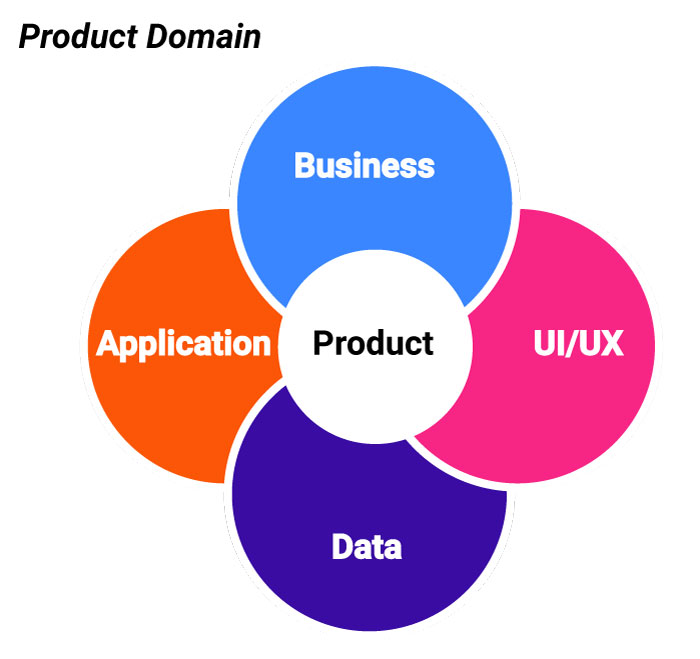
\includegraphics[width=10cm]{Media/product-facets.jpg}
%     \caption{Product Facets}
%     \label{fig:data-facets}
% \end{figure}

However this data-as-a-service model should be carefully implemented to account for explorability, discoverability, security, and quality. The data provided as a service should have the identical qualities to customer-facing products. This also implies, that a product owner should now treat the data facet as an aspect of the product and employ objective measures that assure the desired quality. These measures can be net promoter scores from data consumers, data provenance, and decreased lead time. Product owners, in addition to the application and design aspect of the product, must now incorporate this new facet, and try to understand the needs of the data consumers, how they consume the data, and what are the common tools and technologies to consume the data. This knowledge can help shaping better interfaces for the product.

Product domains may also need to ingest data from upstream domains, and this requires the definition of clear interfaces. Furthermore, each domain should also account for metadata. Metadata is derived from the nature of the product and its data lifecycle. Data can be ingested and served in various forms such as tables, graphs, JSON, Parquet, events, and many more; but in order for the data to be useful for analytical purposes, there is a need to associate data with its corresponding metadata that encompasses semantics, and history.

\subsubsection{Data infrastructure automation}

As the number of product domain increases, the effort required to build, deploy, execute, and monitor services increases. This includes the data pipelines required for that product domain to carry out its functions. The platform skills required for these kinds of work is usually found in Devops engineers and site reliability engineers. Application developers and data engineers are usually not adept at carrying out such workloads in an efficient manner. For this reason, there is a need for highly abstract reusable infrastructural components that can be easily utilized. This implies that teams should be equipped with required infrastructure as a service, that can be easily employed to account for BD needs.

One way to provision such infrastructure as a service, is to utilize infrastructure as a code software tools like Terraform \cite{Terraform} and following the principles of GitOps. Besides, data infrastructure may be extended based on currently running infrastructure for application payloads. However, this might be challenging, as the BD ecosystem is growing rapidly, and while a software application might be running on a EC2 worker node in an EKS cluster on Amazon, the BD system maybe running on Databricks, or using a customer data platform (CDP) solution like Segment \cite{Segment}.This brings the challenge of composing data and application infrastructure together to provide a coherent, cost-efficient and interoperable infrastructure.

Nevertheless, this should not be a daunting task, as one can simply extend the EKS confis and add a new pod to the network, which installs Databricks through a Helm Chart \cite{Helm}. In addition, the data infrastructure should be accompanied with proper tooling. Tools like GNU Make \cite{Make}, makes it quite easy for developers and data engineers to deploy infrastructure as they demand.
A mature infrastructure as a service should provide the team with core infrastructures such as BD storage, stream processing services, batch processing services, event backbones or message queues, and data integration technologies.

\subsubsection{Governance through a federation service}

The other principle of Cybermycelium is the global governance or the global standardization of the services. This principle is perhaps a lesson learnt from the studied application of miroservices architecture in the industry \cite{alshuqayran2016systematic}. Distributed architectures are made up of independent collection of nodes, with distinct lifecycle that are deployed separately and are owned by various teams. As the number of these services grow, and the interconnections increase, the challenge of maintaining and scaling the system increases. This means services need to interoperate, ingest data from other services, perform graph or set operations in a timely manner and do stream processing.

In order to scale and maintain these independently deployed yet interconnected services, Cybermycelium needs a governance model that embrace domain autonomy, decentralization, automation, Devops, and interoperability through federated government. This requires a shift in thinking, which obsoletes many prevalent assumptions of software and data engineering. The point of federation is not to suppress or kill the creativity and innovation of the teams, but rather, introduction of global contracts and standards that are in-line with company's resources and vision. Nevertheless, finding equilibrium between right amount of centralization and decentralization introduces challenge. For instance, semantic related metadata can be left to the product domain to decide, whereas policies and standards for metadata collection should be global. This is somewhat analogous to architectural principles in TOGAF's ADM \cite{josey2016togaf}.

The definition of these standards is up to the architecture, or architectural governance group, and is usually achieved through service level objectives (SLOs) or well-defined contracts and standards.

\subsubsection{Event driven services}

Cybermycelium has been designed in a decentralized and distributed manner. Despite the advantages of decentralized systems in terms of maintenances and scalability, communication between the services remains a challenge. As the number of services grow, the communication channels increases, and this soon turns into a nexus of interconnected services that each try to meet its own end. Each service will need to learn about the other services, their interfaces, and how the messages will be processed. This increases the coupling between services and makes maintenance a challenging task. We argue that this should not be the aim of a distributed RA such as Cybermycelium.

One approach to alleviate these issues is asynchronous communication between services through events. This is a different paradigm to a typical REST style of communication. A point-to-point communication occurs between services as series of `command', like getting or updating a certain resources, whereas event-driven communication happens as a series of events. This implies that instead of service A commanding service B for certain computation, service B reacts to a change of state through an event, without needing to know about service A.

This provides a `dispatch and forget' kind of a model, in which a service is only responsible to dispatch an event to a topic of interest for the desired computation. In this way, the service does not need to wait for the response and see what happens after the event is dispatched, and is only responsible for dispatching events through a well-defined contract. Underlying this paradigm, services do not need to know about each other, but rather they need to know what `topic' they are interested in.

This is analogous to a restaurant, where instead of a waiter needing to communicate directly to another waiter and to the chef and to the cook, they all react to certain events, such as customers coming in, or an order slip being left on a counter. The subtlety lies in the underlying paradigm and philosophy of `event' instead of `command'. This paradigm solves many issues of communication in distributed BD systems such as long running blocking tasks, throughput, maintenance, scale and ripple effect of service failure.

It is worth mentioning, that eventual consistency (BASE) is preferred over ACID transactions for performance and scalability reasons. The detail of these two varying kind of transactions is outside the scope of this study.

\subsection{The Artefact} \label{the-artifact}

After having discussed many kernel and design theories, the necessary theoretical foundation is created for the design and development of the artefact. Cybermycelium is created with Archimate and displays the RA mostly in technology layer. Displaying these services in technology layer means that it is up to the designer to decide what flow and application should exist in each node. For the sake of completion, and as every software is designed to account for a business need, we have assumed a very simple BD business process. While this business layer could vary in different context, Cybermycelium should be able to have the elasticity required to account for various business models. To ease understanding of the RA, we sub-diagrammed the product domain in Figure \ref{fig:Cybermycelium Product Domain Design}.


\subsubsection{Implementation Guide}

Detailed guides, scripts, and configuration templates for system instantiation are hosted in an external repository, providing access to the most recent versions. These materials encompass common setup scenarios and modular integration of components within the Cybermycelium architecture. Complete implementation resources are available at \cite{cybermycelium2023}.


\subsubsection{Components}
Cybermycelium is made up of 11 main components and 9 variable components as depicted in Figure \ref{fig:Cybermycelium}.




% \begin{sidewaysfigure}
%     % \begin{figure}[h!]
%         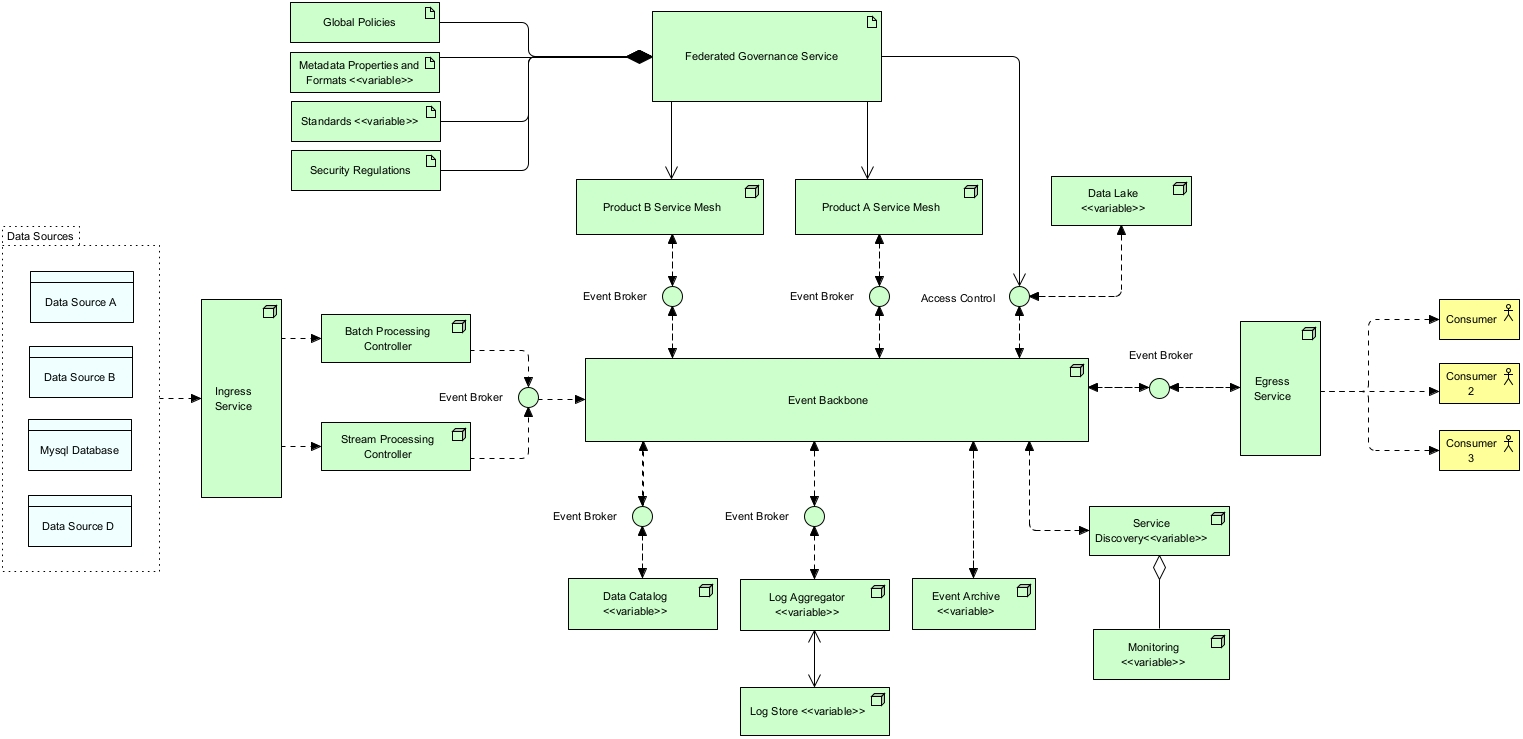
\includegraphics[width=23cm]{Media/Cybermycelium.jpg}
%         \caption{Cybermycelium BD Reference Architecture}
%         \label{fig:Cybermycelium}
%     % \end{figure}
% \end{sidewaysfigure}


% \begin{figure}[h!]
%     \centering
%     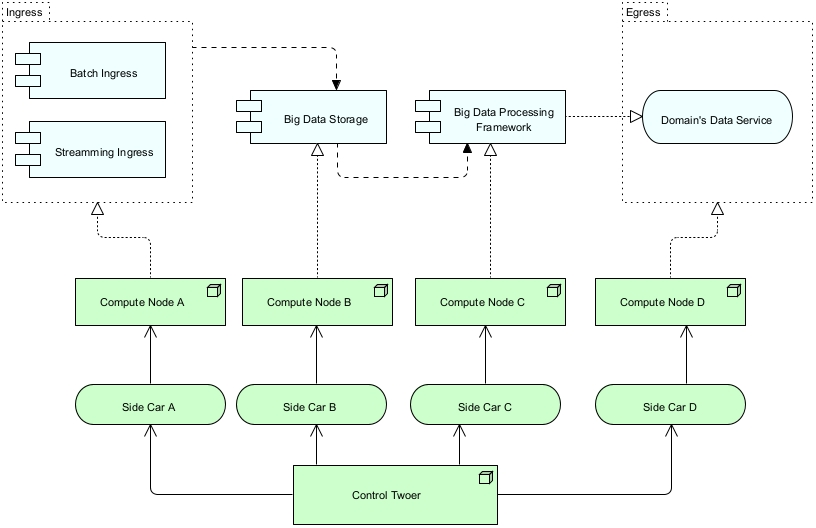
\includegraphics[width=12cm]{Media/Product Domain.jpg}
%     \caption{Cybermycelium Product Domain Design}
%     \label{fig:Cybermycelium Product Domain Design}
% \end{figure}


The main elements are;

\begin{enumerate}
    \item \textbf{Ingress Service:} The ingress service is responsible for exposing the necessary port and endpoint for the data to flow to the system. Depending on the nature of the request, the ingress service will load balance to either batch processing controller or stream processing controller. It is essential for the ingress service to operate asynchronously to avoid any potential choke points. In addition, ingress handles the SSL termination and potentially name-based virtual hosting. Ingress has several benefits. Firstly, it helps with security by preventing port proliferation and direct access to services. Secondly, it help with performance by distributing requests based on their nature, and SSL termination. Thirdly, if there's a need for object mutation through a proxy, ingress is the best architectural construct. Having an ingress also means that the point of entry is clear, which makes monitoring easier, and allows for other components of the architecture to remain in private networks. This component addresses the requirements Vol-1, Vol-2, Var-1, Var-3, Var-4, Val-1, Val-3, Val-4, SaP-1 and SaP-2.

    
    \textbf{Implementation Guide:} For high data throughput or handling sensitive data, it is recommended to employ robust security measures such as SSL/TLS encryption for data in transit, firewall configurations, and rate limiting to protect against Distributed Denial-of-Service (DDoS) attacks. Configuration should adhere to industry best practices for network security and data protection. In smaller-scale implementations or environments with lower security risks, a simplified ingress setup may suffice. This entails configuring the necessary ports and endpoints with appropriate network policies and employing basic SSL termination. Monitoring and logging should be enabled to track the ingress service performance and security incidents. A simple and advanced example of an ingress for Kubernetes can be found in the templates folder at \cite{cybermycelium2023}.

    \item \textbf{Batch Processing Controller:} Batch processing controller is responsible for dispatching batch events to the event backbone. This service should be a small service (could be a Lambda) with the main responsibility of receiving a request for batch processing and dispatching an event to the event broker. Because the nature of the request is of type batch and has been clearly distinguished by the ingress, batch processing controller can dispatch events in bulk and asynchronously. This is the main difference of this service to stream processing controller. Batch processing controller can execute other non compute-intensive tasks such as scrubbing properties from the given data or adding headers. Having a specific controller for batch processing improves monitoring and allows for customized batch event producing. This component addresses the requirements Vel-1, Val-1, and Val-2.
    
    \textbf{Implementation Considerations for Batch Processing Controller:}

    When implementing the Batch Processing Controller, scalability is a primary concern. The service should scale to handle varying volumes of data, possibly through containerization strategies or serverless architectures like AWS Lambda. Error handling and retry mechanisms are crucial to manage failed batch jobs effectively. Integrating comprehensive monitoring and alerting is essential to track job status, performance metrics, and system health. Maintaining data consistency and integrity throughout the processing lifecycle is imperative for ensuring reliable operations.

    \textbf{Variable Components Guidance:}
    
    The Batch Processing Controller is vital for handling large, non-time-sensitive data volumes. However, in environments where real-time or near-real-time data processing is paramount, the emphasis might shift towards Stream Processing Controllers. These controllers are optimized for handling continuous data streams, providing timely insights and responses, and are particularly beneficial in scenarios such as real-time analytics, online transaction processing, or monitoring systems.

    For environments dominated by real-time data needs, transitioning to stream processing involves utilizing technologies like Apache Kafka or Amazon Kinesis, designed for high-throughput, low-latency processing. Sometimes, combining micro-batching with stream processing can balance the need for real-time processing with the efficiencies of batch processing. Effective state management is critical across distributed components in real-time processing systems. Optimizing the entire pipeline for low latency, from data ingestion to processing and eventual action or storage, is essential.

    Whether opting for batch or stream processing, or a hybrid approach, the architecture should align with the specific data, latency, and processing requirements of the application or system. The decision should consider the balance between immediate data handling needs and the efficiencies of batch operations, ensuring that the system is both responsive and efficient.

    \item \textbf{Stream Processing Controller:} Stream processing controller is responsible for dispatching streaming events to the event backbone through the event broker. This service has been segregated from the batch service as it has to account for a different nature of events. Streams are synchronous in nature, and can require high-throughput. This service is a small service as well, but non-heavy computations such as enabling stream provenance, and one-pass algorithms can be utilized. Having a specific controller for stream processing means that custom attributes can be associated to stream events, and the events can potentially be treated differently based on the nature of the system. This also eases monitoring and discovery. This component addresses the requirements Vol-1, Vel-1, Vel-2, Vel-4, Vel-5, Val-2,
    \item \textbf{Event Broker:} Event brokers are designed to achieve `inversion of control'. As the company evolves and requirements emerge, the number of nodes or services increase, new regions of operations may be added, and new events might need to be dispatched. As each service has to communicate with the rest through the event backbone, each service will be required to implement it is own event handling module. This can easily turn into spaghetti of incompatible implementations by various teams, and can even cause bugs and unexpected behaviors. To overcome this challenge, an event broker is introduced to each service of the architecture. Each service connects to its local event broker and publishes and subscribes to events through that broker. One of the key success criteria of the event broker is a unified interface that sits at a right level of abstraction to account for all services of the architecture. Event brokers, being environmentally agnostic can be deployed to any on-premise, private or public infrastructure. This frees up engineers from having to think about the event interface they have to implement and how it should behave. Event brokers can also account for more dynamism by learning which events should be routed to which consumer applications.  Moreover, event brokers do also implement circuit breaking, which means if the service they have to broke to is not available and does not respond for a certain amount of time, the broker establishes unavailability of the service to the rest of the services, so no further requests come through. This is essential to preventing a ripple effect over the whole system if one system fails. This component indirectly addresses the
    requirements Val-1, and Ver-1.
    \item \textbf{Event Backbone:} This is the heart of the Cybermycelium, facilitating communication among all the nodes. Event backbone in itself should be distributed and ideally clustered to account for the ever-increasing scale of the system. Communication occurs as choreographed events from services analogous to a dance troupe. In a dance troupe, the members respond to the rhythm of the music by moving according to their specific roles. In here, each service (dancer) listens and reacts to the event backbone (music) and takes the required action. This means services are only responsible for dispatching events in a `dispatch and forget' model, and subscribe to the topics that are necessary to achieve their ends. Event backbone thus ensures a continues flow of data among services so that all systems are in the correct state at all times. Event backbone can be used to mix several stream of events, cache events, archive events, and other manipulation of events, so long as it is not too smart! or does not become a ESB of SOA architectures. Ideally, an architect should perceive the event backbone as series of coherent nodes that aim to handle various topics of interest. Over the time, event backbone can be monitored for access patterns and can be tuned to facilitate communication in an efficient manner. This component addresses the requirements Vel-1, Vel-2, Vel-3, Vel-4, Vel-5, Val-1, Val-2, Ver-1, Ver-2, and Ver-3.
    \item \textbf{Egress Service:} The egress service is responsible for providing necessary APIs for the consumers of the system to request data in demand. This is a self-serve data model in which data scientists or business analyst can readily request data from various domains based on the data catalogue. Clients can first request for a data catalogue and then use the catalogue to request for the product domain that accounts for the desired data. This request can include several data products. Egress is responsible to route the request to the data catalogue, and to corresponding product `service mesh' in order to resolve values. The egress realizes the address to service meshes and other services through the data catalog and service discovery. The egress service should cache the resolved addresses and values in order to increase performance and response time. An architect can even choose the implement a complete query cache component inside the egress service, however that will incease complexity and can affect modifiability. This component is to avoid having people requesting directly to data engineers for various BD requirements, and means that people can just request for what data they need, analogous to a person who orders food at a restaurant; menu being the data catalog, and egress being the waiter. This component addresses the requirements Vel-2, Vel-4, Val-3, Val-4, SaP-1, and SaP-2.
    \item \textbf{Product Domain Service Mesh:} As previously discussed, a product is a capability of the business, and each product has its own domain consisting of the bounded context and the ubiquitous language. From a system and architectural point of view, these domains are reffered to as a `service mesh'. Each service mesh is made up of a batch ingress, stream ingress, BD storage, BD processing framework, domain's data service, the required compute nodes to run these services, a side car per service and a control tower. These components provide the necessary means for the domain to achieve its ends. This architectural component removes the coupling between the teams and promotes team autonomy. This means people across various teams are enhanced with the desired computational nodes and tools necessary, and can operate with autonomy and scale without having to be negatively affected by other teams or having friction with platform teams or siloed data engineering teams. Depending on the context and the business, the architect may create several domains. This component indirectly addresses Vol-1, Vel-3, Vel-4, Vel-5, Var-1, Var-2, Var-3, Val-1, Val-2, Val-3, Val-4, Sap-1, SaP-2, Ver-1, Ver-2, and Ver-3.
    
    
    \item  \textbf{Federated Governance Service:} Evidently, Cybermycelium is a distributed architecture that encompasses variety of independent services with independent lifecycle that are built and deployed by independent teams. Whereas teams have their autonomy established, in order to avoid haphazard, out-of-control and conflicting relations, there should be a global federated governance that aims to standardize these services. This will facilitate the interoperability between services, communication, aggregates, and even allows for a smoother exchange of members across teams. This also means the most experienced people at a company such as technical leads and lead architects will prevent potential pitfalls that more novice engineers may fall into. However the aim of this service is not centralize control in anyway, as that would be going a step backward into the data warehouse era. The aim of this service is to allow autonomous flow in the river of standards and policies that tend to protect company from external harm. For instance, failing to comply to GDPR while operating in europe can sets forth fines up to 10 million euros, and this may not be something that novice data engineers or application developers are fully aware of. The real challenge of the governance team is then to figure out the necessary abstraction of the standards to the governance layer and the level of autonomy given to the teams. The federated governance service is made up of various components such as global policies, metadata elements and formats, standards and security regulations. These components are briefly discussed below;
    \begin{enumerate}
        \item \textbf{Global Policies:} general policy that govern's the organizational practice. This could be influenced by internal and external factors. For instance, complying to GDPR could be a company's policy and should be governed through the federated governance service.
        \item \textbf{Metadata Properties and Formats:} this is an overarching metadata standard defining the required elements that should be captured as metadata by any service within the organization; it can also include the shape of metadata and the properties of it. For instance, the governance team may decide that each geographic metadata should conform to ISO 19115-1 \cite{ISOMetadata}.
        
        \textbf{Variable Components Guidance:} In the event of deploying an internal application where the data is transient and not subjected to compliance scrutiny, the complexity of metadata can be significantly reduced or omitted. An architect may streamline metadata to essential elements that support basic operational requirements, foregoing expansive metadata schemes typically necessitated by external regulatory bodies.

        \item \textbf{Standards:} overall standards for APIs (for instance Open API), versioning (for instance SemVer), interpolation, documentation (for instance Swagger), data formats, languages supported, tools supported, technologies that are accepted and others.
    
        \textbf{Variable Components Guidance:} In scenarios where a system operates in isolation from external interfaces or in a highly specialized domain with unique requirements, adherence to common standards may be relaxed or omitted. The architect must ensure that any deviation from established standards does not impede future integration efforts or system scalability. The decision to omit standardization should be deliberate, with a focus on maintaining system agility while safeguarding against potential technical debt.
    
        \item \textbf{Security Regulations:} company wide regulations on what's considered secured, what softwares are allowed, how interfaces should be conducted and how the data should be secured. For instance, company may choose to alleviate risks associated with OWASP top 10 application security risks.
    \end{enumerate}

    While we promote above mentioned components as bare minimum, an architect may decide to omit or add a few more components to the federated governance service. This component can indirectly affect all requirements.

    \item \textbf{Data Catalog:} As the products increases, more data become available to be served to consumers, interoperability increases, and maintenance becomes more challenging. If then, there is no automatic way for various teams to have access to the data they desire, a rather coupled and slow BD culture will evolve. To avoid these challenges and to increase discoverability, collaboration, and guided navigation, the service data catalog should be implemented. Data catalog is listed as a must-have by Gartner \cite{GartnerDataCatalog} and introduces better communication dynamics, easier data serve by services and intelligent collaboration between services. This component addresses the requirements Vel-4, Var-1, Var-3, and Var-4.
    
    \textbf{Variable Components Guidance:} In scenarios where the organization utilizes a single or limited number of data sources, the structure of the data catalog could be condensed or entirely omitted. The architect could pivot towards a direct query approach against the source systems, especially in environments where data lineage and sourcing are not of paramount concern.
    
    \item \textbf{Logging Aggregator and Log Store:} If all services employ the idea of localized logging, and simply generate and store logs in their own respective environments, debugging, issue finding and maintenance can become a challenging task. This is due to the distributed nature of Cybermycelium and the requirements to trace transactions among several services. In order to overcome this challenge, we have employed the log aggregator pattern popularized by Chris Richardson \cite{MicroServicesPatterns}. The log aggregator service is responsible for retrieving logging events through the event broker from individual services and writing the collected data into the log store. The log aggregator configuration and semantics is up to the designer and architecture team. This allows for a distributed tracing, and graceful scaling of organizational logging strategies. This component indirectly addresses the requirements Vol-1, Vel-1, Val-1, and Ver-1.
    
    \textbf{Variable Components Guidance:} For applications with a narrow scope of operation and minimal user base, such as a prototype or an internally-used tool, the logging aggregator may be omitted. In such cases, direct log analysis methods may suffice, freeing the system from the additional layer of log aggregation complexity.

    \item \textbf{Event Archive:} As the quantity of services grow, the topics in event backbone increases, and the number of events surges. Along the lines of these events, there could be a failure, resulting in timeout and a loss of series of events. This brings system in a wrong state and can have detrimental ripple effect on all services. Cybermycelium tends to handle these failures by using an event archive. The event archive as the name states, is responsible for registering events, so they can be retrieved in the time of failure. If there was a blackout in certain geographical location and the event backbone went down, the backbone can recover itself and bring back the right state of the system by reading the events from the event archive. Th event broker is responsible for circuit breaking, so services do not request any more events to the backbone while its down. The time to expiry, and what events should be archived is decided based on context in which Cybermycelium is implemented. This component indirectly addresses
    the requirements Vol-1, Vel-1, Val-1, and Ver-1.

    \textbf{Variable Components Guidance:} In a development or testing environment where events are non-critical, the event archive could be omitted. The architect might determine that the operational overhead of maintaining an archival system outweighs its benefits in a non-production scenario.

    \item \textbf{Data Lake:} Whereas Cybermycelium is a great advocate of decentralized and distributed systems, we do not find it necessary for each product domain to have its own kind of a data lake or data storage. This is to prevent duplication, contrasting data storage approaches, decreased operability among services and lack of unified raw data storage mechanisms. Data lake has been designed to store large volume of data in raw format before it can get accessed for analytics and other purposes. This means data can be first stored in the data lake with corresponding domain ownership before it needs to be accessed and consumed by various services. Structured, semi-structured, unstructured and psudo-structured data can be stored in data lake before it gets retrieved for batch and stream processing. Nevertheless, this does not imply that all data should directly go to the data lake; the flow of data is determined based on the particularities of the context in which the system is embodied. One approach that we find suitable is for each team to own a unit of storage in the data lake, which is handled by the access control. This component addresses the requirements Vol-2, Vel-1, Var-1, Var-3, Var-4, Val-3.
    
    \textbf{Variable Components Guidance:} A scenario that warrants the omission of complex partitioning strategies within the data lake is when the enterprise operates on a small-scale data footprint with homogeneous data types. Here, an architect may favor a simplified, flat-storage approach, eliminating the need for elaborate partitioning and the overhead it entails.
    

    \item \textbf{Service Discovery:} In a distributed setup like Cybermycelium, how do services discover the location of other services? This is achieved through service discovery. As the practice of hard-coding service addresses in configuration files is not a maintainable or scalable approach, one has to think about an automated scalable solution in which services can become discoverable by other services. The service discovery node is responsible for this job. This is achieved through services registering themselves to the service discovery node when they boot up. Service discovery then ensures that it keeps an accurate list of services in the system, and provides the API necessary for others to learn about the services. For instance, it is idiomatic for an engineer to specify a command to be executed when a Docker container starts (\emph{Node server.js}); thus one can imagine extending the boot up instructions to achieve the registration to the service discovery node. This somewhat resembles to DHCPs and house wifi networks.  This component indirectly addresses the requirements Vel-2, Vel-4, Var-2, Var-4, Val-3, Val-4, SaP-2.
    
    \textbf{Variable Components Guidance:} For monolithic applications or when services are statically assigned and do not require discovery for communication, the service discovery component can be omitted. An architect might bypass this component to reduce architectural complexity in a stable and predictable deployment environment.

    \item \textbf{Monitoring:} Monitoring systems are integral to robustness of highly dynamic ecosystem of distributed systems and directly affect metrics such as mean time to resolution (MTTR). Services emit large amounts of multi dimensional telemetry data that covers a vast spectrum of platform and operating system metrics. Having these telemetry data captured, handled and visualized, helps systems engineers, software reliability engineers, and architects proactively address upcoming issues. Based on these premises, the main responsibility of this service is to capture and provide telemtry data from other services to increase the overall awareness of the Cybermycelium ecosystem. This service is tightly aggregated with the service discovery. Monitoring services help storing these data to fuel proactive actions. This component
    indirectly addresses all requirements.

    \textbf{Variable Components Guidance:} In smaller, less complex systems where the operational state can be ascertained without extensive monitoring, an architect may decide to omit advanced monitoring configurations. This could apply to single-service applications or ones with minimal integration points, where basic monitoring suffices.

\end{enumerate}

\subsubsection{Variable Components}

The variable elements in Cybermycelium can be adjusted, modified and even omitted based on the architect's decision and the particularities of the context. The aim of this RA is not limit the creativity of data architect, but to facilitate their decision making process, through introduction of well-known patterns and best practices from different school of thoughts. While we still recommend keeping the variable components, an architect may decide to embark on a more complicated metadata approach rather than just a data catalog. We do not elaborate on all alternative options for each variable module as industry constantly changes, and architects constantly aim to design systems that address the emerging problem domains. 

\subsection{Decision-Making Aid}

The Component Decision Tree illustrated in \ref{fig:decisionMakingTree} is designed to guide architects through the intricate process of selecting, modifying, or omitting various components based on a multitude of factors. This tool addresses the architectural flexibility and varying application scenarios, providing a structured pathway to informed architectural choices.

Developed through an analysis of the architecture's components and influenced by factors such as data volume, system complexity, and compliance needs, the tree presents decision nodes leading to multiple pathways. These nodes represent key architectural considerations, directing the implementation towards a configuration that aligns with organizational objectives and technical requirements. Architects begin with an assessment of the organizational context, which influences the direction and complexity of subsequent decisions. As they traverse the tree, they engage with decisions concerning data scale, processing needs, security, compliance, and scalability, each with its ramifications and trade-offs.

The dynamic nature of technology and enterprise needs means the Component Decision Tree is not static but an evolving tool, adaptable to new insights and changing requirements. it is meant to be integrated into the Cybermycelium documentation, offering a navigable and intuitive guide for architects and stakeholders. Regular updates and refinements ensure its relevance and applicability in guiding towards a robust, scalable, and efficient architecture.

% \begin{figure}[!h]
%     \centering
%     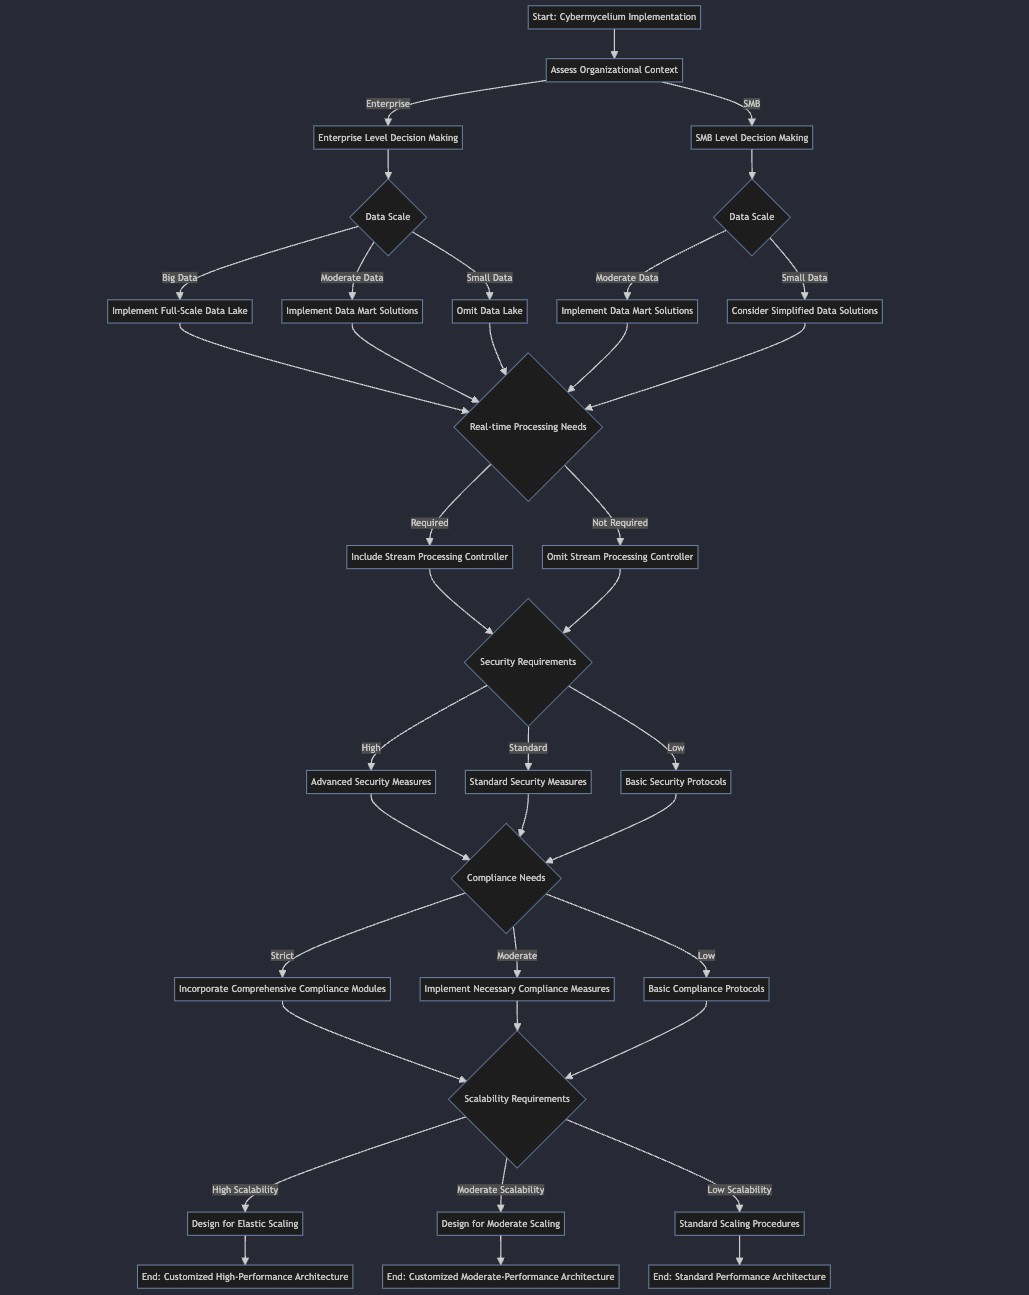
\includegraphics[width=10cm]{Media/Decision-making-tree.png}
%     \caption{Decision Making Tree for Cybermycelium}
%     \label{fig:decisionMakingTree}
% \end{figure}

\subsection{Conclusion}


The aim of this RA is not to limit the creativity of the data architect but to facilitate their decision-making process through the introduction of well-known patterns and best practices from different schools of thought. While we still recommend keeping the variable components, an architect may decide to embark on a more complicated metadata approach rather than just a data catalog. We do not elaborate on all alternative options for each variable module as industry constantly changes, and architects constantly aim to design systems that address the emerging problem domains. 



\section{Evaluation:} \label{evaluation-section}

Of particular importance to development of a RA, is the evaluation of it. As previously discussed, our aim is to evaluate the RA's correctness and utility by assessing its transformation into an effective, context-specific concrete architecture, following the guidelines of ATAM. The main goal of ATAM is to appraise the consequences of architectural decisions in light of quality attributes. This method ensures that the architecture is under the right trajectory and in-line with the context. Architecture is a amalgamation of risks, tradeoffs, and sensitivity points. Using ATAM increased our confidence by uncovering key architectural tradeoffs, risks, and sensitivity points.

For ATAM to be successful there should not be a precise mathematical analysis of system's quality attributes, but rather trends should be identified where architectural patterns are correlated with a quality attribute of interest. For brevity purposes, we do not expand on what ATAM is, and the details of each steps in it, and we only explain how the evaluation has been conducted through ATAM. It is important to note that, this wasn't a setup in which an outside evaluation team would come to a company to evaluate an architecture in practice, but it was our prototype that we brought into a company to test its utility and relevance. 

While we could have achieved this with technical action research or lightweight architecture evaluation, we found ATAM to be in-line with our conceptual constructs, which are architectural constructs. ATAM provided us with a framework to discuss architectural concepts in a rigorous way \cite{wieringa2014design}. We created the prototype, and played the role of the evaluator, thus there was a risk of bias. To avoid bias, we invited a third-party researcher who is familiar with ATAM to observe the overall process and partake in architectural probing questions. 

For instantiation of the RA, We utilized ISO/IEC 25000 SQuaRE standard (Software Product Quality Requirements and Evaluation) \cite{ISO25000} for technology selection.  We did not fully adopt this standard, but were rather inspired by it to make a better decision. The quality model in the standard is based on characteristics, sub-characteristics and standards.


The technology research phase combined a structured literature review with hands-on exploratory testing, ensuring a comprehensive understanding of potential technologies for the Cybermycelium architecture. The literature review delved into academic papers, industry reports, product documentation, and user testimonials to understand various technologies' theoretical underpinnings, practical applications, strengths, and limitations. This phase was essential in assessing the alignment of each technology with the specific requirements of Cybermycelium.

Concurrently, exploratory testing provided firsthand insights into the functionalities, maintainability, compatibility, and portability of the technologies. This practical examination ensured that each technology was rigorously assessed against established evaluation criteria, with findings documented for subsequent analysis. Following the research, a detailed evaluation matrix (see Section~\ref{TechnologyEvaluationMatrix} in Appendix) facilitated a comparative analysis of each technology's performance, enabling a nuanced comparison. Technologies were scored based on criteria such as Functional Suitability, Maintainability, Compatibility, and Portability, leading to a comprehensive understanding of their overall suitability for the architecture.

We chose the tools are the mostly adopted and do support the architectural requirements of Cybermycelium. We did not want to develop tools from scratch, as that would delay our evaluation artefact and this would affect the stakehodlers negatively. In addition, many mature tools exist that statisfy our architectural requirements, so therefore `reinventing the wheel' was unnecessary. Table~\ref{tab:components-tech-req} is the breakdown of how each technology was implemented in the Cybermycelium prototype:

\begin{table}
    \centering
    \begin{tabular}{|p{3.5cm}|p{3cm}|p{5cm}|}
    \hline
    \textbf{Component} & \textbf{Technology} & \textbf{Requirements Addressed} \\
    \hline
    Ingress Service & Nginx & Vol-1, Vol-2, Var-1, Var-3, Var-4, Val-1, Val-3, Val-4, SaP-1, SaP-2 \\
    \hline
    Batch Processing Controller & AWS Lambdas & Vel-1, Val-1, Val-2 \\
    \hline
    Stream Processing Controller & AWS Lambdas, Kafka Streams & Vol-1, Vel-1, Vel-2, Vel-4, Vel-5, Val-2 \\
    \hline
    Event Broker & Kafka & Val-1, Ver-1 (indirectly) \\
    \hline
    Event Backbone & Kafka & Vel-1, Vel-2, Vel-3, Vel-4, Vel-5, Val-1, Val-2, Ver-1, Ver-2, Ver-3 \\
    \hline
    Egress Service & AWS Application Load Balancer, Node JS & Vel-2, Vel-4, Val-3, Val-4, SaP-1, SaP-2 \\
    \hline
    Product Domain Service Mesh & Istio, Envoy & Vol-1, Vel-3, Vel-4, Vel-5, Var-1, Var-2, Var-3, Val-1, Val-2, Val-3, Val-4, SaP-1, SaP-2, Ver-1, Ver-2, Ver-3 \\
    \hline
    Data Lake & AWS S3 & Vol-2, Vel-1, Var-1, Var-3, Var-4, Val-3 \\
    \hline
    Event Archive & AWS S3 & Vol-1, Vel-1, Val-1, Ver-1 (indirectly) \\
    \hline
    \end{tabular}
    \caption{Components, Technologies, and Requirements in the Cybermycelium Evaluation}
    \label{tab:components-tech-req}
\end{table}

% \begin{sidewaysfigure}
%     % \centering
%     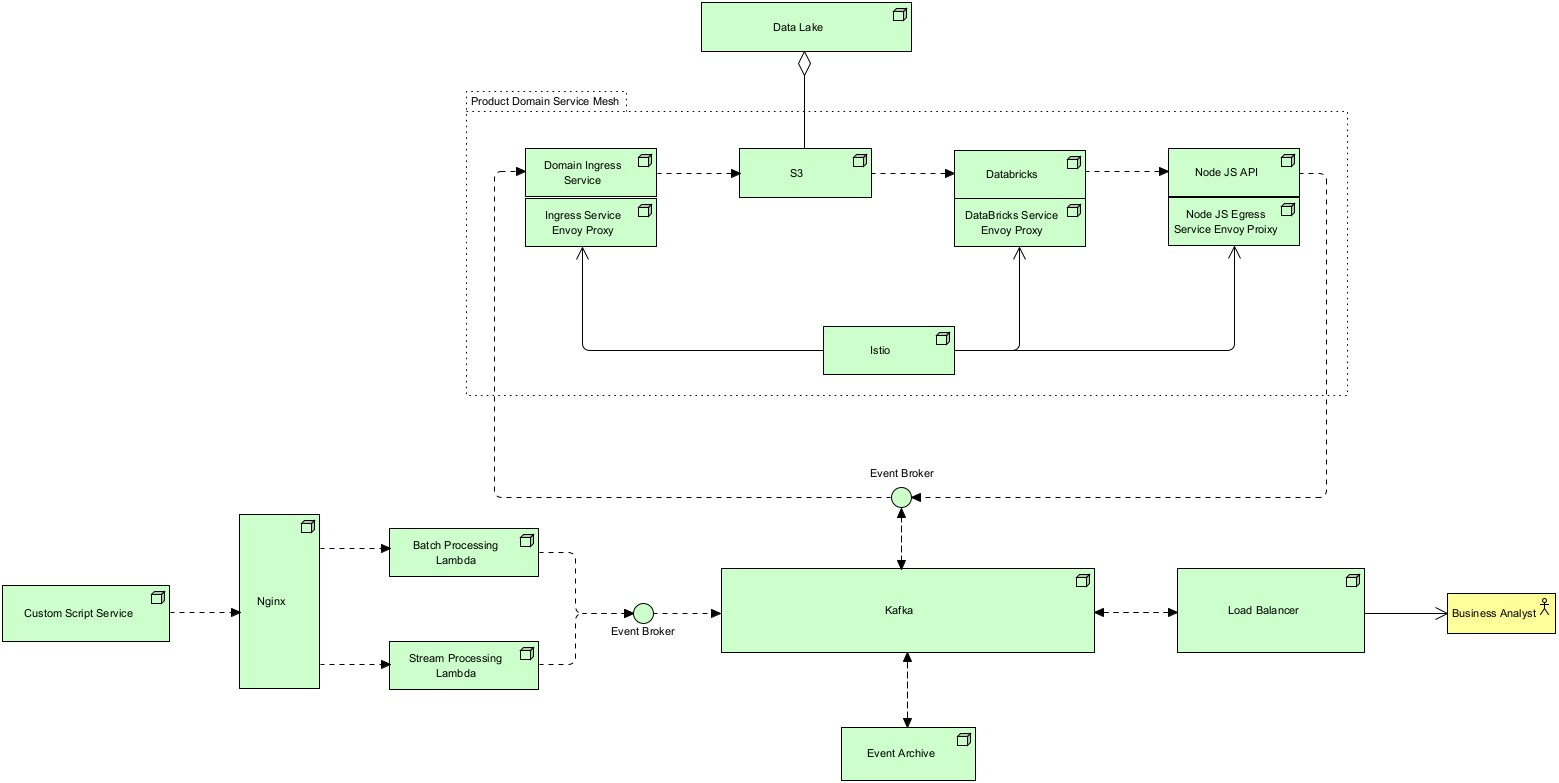
\includegraphics[width=23cm]{Media/concrete-mycelium.jpg}
%     \caption{Cybermycelium Instantiation}
%     \label{fig:ConcreteCyberMycelium}
% \end{sidewaysfigure}

We aimed to incorporate most components of our RA into this instance, however logging, monitoring, service discovery, federated governance service, and data catalog has been omitted. Some details of this evaluation is omitted to protect the security, and intellectual property of the practice, and some details are modified for academic purposes. These modifications have not affected the integrity of the evaluation. This evaluation is an iterative process, collecting feedback from different group of stakeholders in each phase. 

\subsection{Phase 1:}

This evaulation is undertaken in a subsidiary of a large-scale international company that has over 6000 employees all around the globe. The subsidiary company offers a pratice management software for veterinary practitioners via Software as a Service (Saas) and has over 15,000 customers from the USA, UK, Australia, New Zealand, Canada, Singapore and Ireland, among which are some of the biggest equine hospitals, universities and veterinary pracices. The company is currently at the stage of shifting from centralized synchronous architecture into decentralised event driven microservices architecture, and is ambitious to adopt artificial inteligence and BD.

The initial step was the identification ot relevant stakeholders. For this purpose we have approached the key stakeholders in the company's technical governance team. Our aim was to incorporate at least two lead architects of the company in this process. We emphasized on architects that have been with business for a long period of time. This was to ensure that we do not miss any important element in the process of evaluation. As a result, we invited two lead development architects, head of product, and a business analyst for phase 1.


\subsubsection{Step 1 and 2: Introduction}

During the initial meeting, in step 1, ATAM was presented with clear description of its purposes. In step 2, stakeholders discussed the background of the business, some of the challenges faced, the current state of affairs, the primary business goals, and architecturally significant requirements. This step illuminated on integral elements such as: 1) most important functions of the system, 2) any political, regional, or managerial constraints, 3) the business context and how it relates to our prototype, 4) architectural drivers.


\subsubsection{Step 3: Present the Architecture}

In step 3, the prototype has been presented, our assumptions have been stated, and variability points portrayed. 

\subsubsection{Step 4: Identifying Architectural Approaches}

To establish the architectural styles, we first analyzed the prototype with regards to architectural patterns and princinples depicted in Section~\ref*{theory-section}. We then digged a bit deeper and justified our architectural decisions. We discussed the event-driven nature of the prototype, and discussed the usefulness of the domains.

\subsubsection{Step 5: Utility Tree Elicitation:}
In order to generate the utility tree, first we had to learn what are the most important quality attributes. While we learnt about these quality attributes in step 2 shortly, in this step we probed deeper. We first presented our assumptions, and double-checcked it with the stakeholders. Whereas some stakeholders raised concerns over privacy, the members unanimously agreed that performance, availability, and maintainability are the most important quality attributes. This was in-line with our assumptions. In this process, we rated the technical difficulty, and the key stakeholders rated the business importance.

Based on these premises, the utility tree has been generated (Figure \ref{fig:utility-tree} ). Each node on the utility tree corresponds to specific real-world scenarios, linking quality attributes to measurable outcomes. This ensures that performance, availability, and modifiability are tested against the day-to-day operations of the SaaS environment.

In addition to identifying the key quality attributes, we elicited specific scenarios to test these attributes within the context of our SaaS company's operational environment. Each scenario was designed to rigorously test the Cybermycelium architecture against the metrics defined in the utility tree. The scenarios include:

\begin{itemize}
    \item \textbf{Scenario 1:} Real-time processing of streaming data from multiple clinics, with the system maintaining response times under 1200ms even during peak usage.
    \item \textbf{Scenario 2:} Simulated failure of a data center to test the resilience of the load balancer and the cluster availability, maintaining 99.99\% and 99.999\% uptime respectively.
    \item \textbf{Scenario 3:} Integration of a new third-party service within a week, showcasing the modifiability and extensibility of the service mesh infrastructure.
    \item \textbf{Scenario 4:} Addition of new data sources in response to changing privacy regulations, completed within the modifiability goal of less than one week.
\end{itemize}

 These scenarios provide a broad overview of the types of challenges and requirements the architecture must address. They serve as foundational concepts that will be further refined into more specific and detailed scenarios in subsequent steps of the ATAM process.

% \begin{figure}[h!]
%     \centering
%     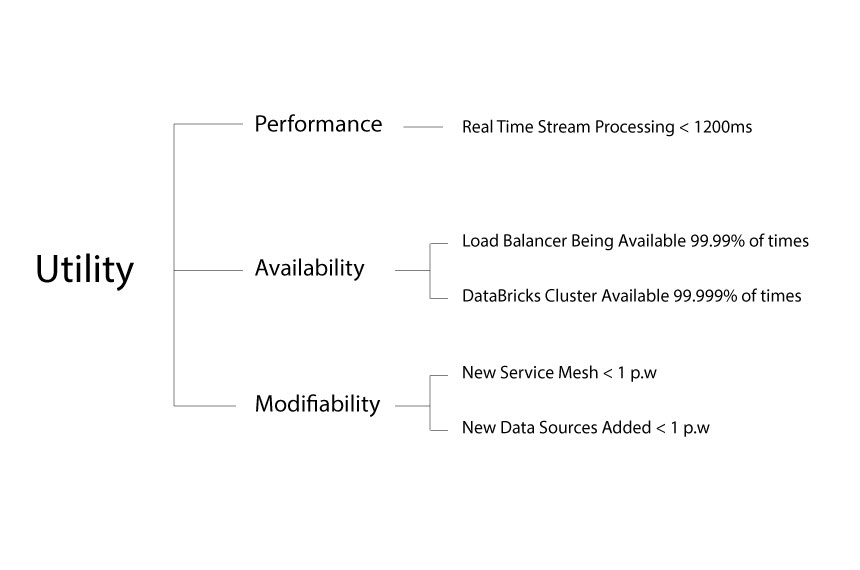
\includegraphics[width=10cm]{Media/Utility-tree.jpg}
%     \caption{Utility Tree}
%     \label{fig:utility-tree}
% \end{figure}

\subsubsection{Step 6: Analyze Architectural Approaches:}

Prior to commencing this step, we conducted simulations of the prioritized scenarios against our prototype to validate the architecture's response against our utility tree metrics. These simulations provided valuable insights into the system's performance under various stress conditions and its ability to adapt to new requirements rapidly. 

After this, analysis of the architectural approaches took place. In this step, we asked the lead architects to probe the architecture and we explained how the prototype is addressing each scenario. 

We justified our architectural constructs by evaluating key quality attributes we have collected previously for the purposes of this evaluation. We explained the following for each quality attribute:

\begin{itemize}
    \item For performance, Nginx, Kafka, Istio, DataBricks and the AWS Application Load Balancer have been described.
    \item For availability, Kafka, Event archive, Nginx, controllers, Data Lake and Istio have been discussed.
    \item For modifiability, the concept of domain-driven design, the service mesh, zere coupling, the plug and play nature of the archetype, the ability to add desireable services through event brokers, and the distributed nature of the architecture has been discussed.
\end{itemize}

The result of this step, was identification of sensitivity points, trade-offs, risks and non-risks. This step took longer than what we anticipated, as variety of questions arose and many aspects of the architecture was challenged. The detail is discussed in Section~\ref{evaluation-results}. 
 

\subsection{Phase 2:}

This phase was a more serious phase of our evaluation, as we invited more stakeholders, collected more scenarios and even created simulations. For this phase, in addition to lead architectes, we invited a product owner responsible for the product in which the artefact is tested, a quality assurance engineer and several developers. We repeated step 1, and provided with recap of step 2 to 6, and shared the current list of risks, non-risks, sensitivity points, and tradeoffs. 

This phase is an iteration of phase one, so we collected scenarios, analyzed architectural approaches, and finally presented the result of the evaluation. 

\subsubsection{Step 7: Brainstorm and Prioritize Scenarios}

Building upon the high-level scenarios defined in Step 5, this step involves a detailed brainstorming session to develop specific, context-driven scenarios. These refined scenarios provide a fine-grained and realistic set of challenges and opportunities that the Cybermycelium architecture must address, reflecting the unique operational environment of the SaaS company. They are designed to be direct derivatives of the broader concepts introduced earlier, now tailored to test the system's responses in a more rigorous and precise manner.


Based on this premise, in this step, we asked stakeholders to come up with three different kind of scenarios namely growth scenarios (anticipated changes), use-case scenarios (typical usage of the system) and exploratory scenarios (extreme cases). The result of this created 20 scenarios, which we then asked stakeholders to vote on. Drawing from the quality attributes highlighted in the utility tree, stakeholders were prompted to conceive scenarios that test the system's capabilities in a pragmatic setting. The following scenarios were derived, each tailored to challenge and assess the architecture's response to realistic operational demands:

\begin{itemize}
    \item \textbf{Scenario 1:} "Rapid Diagnostics Turnaround" - In the context of a veterinary hospital, the architecture must support the real-time analysis of lab results, enabling a diagnosis for conditions like Lyme disease within a critical time window, ensuring that response times remain below the threshold of 1200ms.
    \item \textbf{Scenario 2:} "Disaster Recovery" - A simulation of a regional data center outage tests the system's failover mechanisms, specifically the ability of the load balancer and data cluster to maintain operational availability above 99.99\%.
    \item \textbf{Scenario 3:} "Seamless Integration" - The architecture must facilitate the integration of a new third-party service mesh within a week, demonstrating the system's adaptability to evolving business partnerships and technical ecosystems.
    \item \textbf{Scenario 4:} "Compliance Adaptation" - In response to updated privacy regulations, the system must accommodate the addition of new data sources and changes to data handling processes within a week, showcasing the architecture's modifiability and compliance agility.
\end{itemize}

In turn, these scenarios are described as two user journeys;

\begin{itemize}
    \item A cat owner brings a cat to the veterinary hospital. The cat has symptoms of a lyme disease, and should be diagnosed in a timely manner to avoid master problems.
    \item There has been numerous cases of cancer in pets in certain environments. This environment should be analyzed to see if environmental factors play a cancer inducing role.
\end{itemize}

\subsubsection{Step 8: Analyze Architectural Approaches}

Before starting this step, we took a few days break to simulate the scenarios against our prototype. While ATAM does not prescribe this, we augmented our evaluation with this simulation to ensure that we do not overlook any necessary architectural detail. This improved our confidence in our RA and the architectural probing questions to come. 

We emulated the scenarios against the prototype by creating relevant topics in the Kafka, having the data flow, having the ingress in the service mesh digest it and flow it into the storage and processing and so on so forth. we have been using real world data, so there was no need for data fabrication and synthesis. We configured Nginx to pass the request to the responsible Lambdas, and Lambdas then produced the necessary events and sent it to Kafka. 

We presented our simulation alongside some metrics we captured and displayed in our cloud served Garafana instance. From here on, this step followed the exact same procudure as step 6, with a difference that this time there's been more extensive probing and analysis of the architecture and the simulated scenarios. The simulation and results of it helped clarifying on some of our architectural constructs and led to emergence of several questions: 

\begin{itemize}
    \item How does the system reocover if the event backbone goes out of order?
    \item What if the service mesh ingress is not available?
    \item Should privacy be it is own service? or should it sit in federation ?
    \item Should have a dedicated service mesh for metadata management?
    \item How easy it is to extend and modify current services?
    \item Should there be a certain order to events ?
    \item Is there a benefit in creating event mesh between event brokers?
    \item Where is the best place to scrub sensitive data from the incoming streams?
\end{itemize}

\subsubsection{Step 9: Present Results} \label{evaluation-results}

In this last step, the collected theories form the process of evaluation is discussed in terms of quality attributes, risks, sensitivity points, tradeoffs and other unplanned discussions that arose during the meetings. 

Based on the result of our evaluation, stakeholders feedback, utility tree, and the architectural qualities of Cybermycelium, we deduce that system quality Q\textsubscript{S}, is a function f of the quality attributes availability Q\textsubscript{A}, performance Q\textsubscript{P}, and modifiability Q\textsubscript{M}.

\begin{equation}
    Q\textsubscript{S} = f(Q\textsubscript{M}, Q\textsubscript{A}, Q\textsubscript{P})
\end{equation}

\paragraph{Performance} In order to analyze our approach in-line with the utility tree, after having created the simulated scenarios, we used a cloud stress testing testing agent (StressStimulus). After having run this stess test a couple of times, it has become evident to us that cold start latency of AWS Lambda services can affect the performance requirements stated in the utility tree. A Lambda can take anywhere from 100ms to over a second on cold start time. This latency varies and hard to nail down, but even considering the latency, we have captured an average of 1000ms response time from our system which is inline with the utility tree. While replacing Lambdas with EC2s or Fargates could solve this issue, it would increase the cost, affect the maintainbility of the architecture (a server has to be provisioned and maintained), and would require rework of several services.

In addition, other Lambda like solutions exist that have actually sovled the cold start problem; one good example is cloud workers offered by CloudFlare. However the company chosen for the purposes of this evaluation is not yet open to a multi-cloud approach, and thus AWS is the only option. Moreover, one could implement predictable start-ups with provisioned concurrency, but that requires more effort and is outside the scope of this study. As our architecture is distributed, we have also measured the latency in between services as tail latency is a known issue in distributed systems. Due to the fact that our service mesh was hosted in a private network on a virtual cloud, we could not find any major issue with cloud latency, and our average response time was under 1000ms. Implementing a streaming processing in Databricks, we opted not to use micro-batch to have an accurate evaluation, and we decided not to configure the fair scheduling pool, so as to test the worst case scenario.

After creating and analyzing various performance models of the system, it has come clear to us that latency, and side-effects like input/output, and mutation/transformations were the most important performance sensitivity points. Our performance model were built underlying the following cases;

\begin{itemize}
    \item Priodic, regular data dispatch to the product domain
    \item Sending large volume of data (over 200mb) to the system, reaching the throughput threshold
    \item Sending many request simutaneously through the cloud stress testing tool
\end{itemize}

The event-driven nature of the system really helped with handling throughput and concurrency. Whereas there has been bottlenecks in the areas of storage and network latency, the system managed to reach desired performance on average. Given this insight and after some rigorous testing, we characterize the system's performance sensitivity as follows;

\begin{equation}
    Q\textsubscript{P} = h(s, l, cbp)
\end{equation}

That is the system is sensitive to side effects (s), latency (l), and concurrency back pressure (cbp).

\paragraph{Availablity:}

As guided by the utlity tree, the key stimulus to model for the prototype is the failure of the ingress (load balancer), the data processing cluster and most importantly the event backbone. Due to the distributed nature of Cybermycelium, and the derived prototype, failure in one service, if not handled properly, can have a ripple effect on the system. This is one area, where we found the idea of 'event brokers' really helpful. By implementing circuit breakers in event brokers, we prevented the other nodes of the system to be affected by failure of one. We also archived the events that the node was about to receive before it failed.

Whereas the event archive has played an ancillary role in providing archive to various circuit breakers, it is main functionality was to provide event history to the event backbone in the case of failure. This is again achieved by circuit breaking at the broker level and event retrieval from the event archive. On the other hand, in relation to container orchestration and health check, Kubernetes provided with a declarative API to handle the state of the system. With setting replica sets, and necessary deployments, the master node kept ensuring that certain number of pods are always available. This implies that it is critical for master node to be available at all times.

Based on these findings, we characterized system's availability as following (g is fraction of time that system is working);

\begin{equation}
    Q\textsubscript{A} = g(\lambda\textsubscript{E} , \mu\textsubscript{C}, \mu\textsubscript{S})
\end{equation}

That is, system availablity is primarily affected by the failure rate of the event backbone ($\lambda \textsubscript{E}$), the time it takes for circuit breaker to trip and become available again ($\mu\textsubscript{C}$), and the time it takes for the service to recover from failure ($\mu\textsubscript{S}$).

One major factor that really helped alleviating many issues of the distributed systems, was the cloud-native aspect of Cybermycelium. Whereas this aspect of the architect has not beed discussed previously, the prototype was easily deployed in AWS with well-known Amazon web sevices. As we did not handle on-premise data centers, many of the hardware was handled by the cloud company.

\paragraph{Modifiability:}

To analyze modifiability, we followed the guidelines of SAAM \cite{kazman1994saam}. The distributed and service driven nature of the prototype allowed us to easily achieve the utility tree and even further. All of our cloud based infrastructure has been written as Terraform code in HCL, which meant adding a new node in the system, was as easy as copying the worker groups block in the EKS configuration, and setting the hardware properties of it. We could then easily deploy different services and deployments and have them run our public docker images. Brokers were also streamlined, and we could spin up a new broker within minutes. One area that we found a bit challenging to modify was perhaps the Databricks cluster, and the EKS ALB ingress (Nginx).

Certification management was also easily handled through Istio, local CertManager and Let's encrypt. One area that could be taking a bit longer was the inclusion of private docker image secrets as a Kubernetes secret, and having it refreshed every 12 hours. To the best of our knowledge, cron jobs were the only way to achieve this, but the implementation was not straight forward.

On the other hand, bringin up a scalable Kafka cluster was not that difficult, but there were so many configurations that one can choose to turn on or amend. This can potentially affect modifiability in the long run, when the company might have varying and sometimes conflicting requirements.

Modifiability is also affected by the skillset of the engineers and how familiar they are with Kubernetes, Databricks and Istio. Taking all these into consideration, we characterize system's modifiability as follows (s is the skill set required);

\begin{equation}
    Q\textsubscript{M} = s(K, D, K)
\end{equation}

That is, the system modifiability is affected the Kubernetes maintenances (K), Databricks maintenances, versioning and configuration (D), and Kafka versioning, maintenance and configuration.


\paragraph{Tradeoff Points:}

As a result of these analyses, we identifed two tradeoff points;

\begin{enumerate}
    \item Event backbone and event brokers
    \item Service mesh
\end{enumerate}

One area that arose many worries is the event backbone. Event backbone being the communication facilitator has raised a lot of questions and many worried that this might turn into a bloated architectural component like enterprise service bus (ESB) in the service oriented architectures (SOAs). We addressed many of these questions and issues both in a dicussion and the prototype. Implementing event archive meant that if the event backbone went down, we could restore the previous state of affairs and bring services to the correct state. The implementation of circuit breakers through the event brokers further solidifed the avaiability of the architecture and could deem to affect reliability too. Along the lines, event brokers helped us address some of the modifiability challenges. Having these event brokers setup, meant that different environments do not implement their own event processing mechanism, and the interface is unified across. This clear interface contributed positively to the overall modifiability of the system and allowed engineers to simply copy the broker for their services. In addition, brokers also improved interoperability, and hard to trace bugs duge to event processor missmatch.

Given all, Cybermycelium does not tend to dictate what has to be done, or kill the creativity of the archites, but rather aims to shed ligts on a novel perspective to designing BD systems. Therefore, the event backbone and event brokers introduce tradeoff between performance, availability and reliability. Whereas eliminating the event backbone may increase avaiability longitudinaly, and increase modifiability cross-sectionally, it may affect the performance quality attribute in a negative way. This is due to the fact that the event backbone is distributed in nature, can scale well to account for demans, can cache and remember communication paths, merge event streams, provide with windowing techniques, and be configured to facilitate certain access patterns that are common to the system.

Anothe area where stakeholders were challenged was the idea of service mesh. Whereas this makes a lot of sense to developers who had to figure out the twisted platform work, the benefit perhaps was not that evident to everyone from the beginning. This is another area of tradeoff. While having the service mesh affects the modifiability of the system in a negative way from platform point of view, it does increase it from data engineering and software engineer point of view. The service mesh may also affect performance slightly, but the effect is negligible. Service mesh also affects avaiability positively by streamlining the platform interfaces, providing an orchestrator ( control tower ), and doing health checks through proxies.

\paragraph{Limitations}

Cybermycelium is a new perspective to BD system development and tends to absorb many of the well-established patterns and ideas from various domains. Being distributed in nature, there are still many areas in which Cybermycelium can improve. For instance, we still don't have a great answer to tail latency issues which can affect system negatively. Besides that, we recived feedbacks that many developers find Cybermycelium a complex architecture that require a lot of skill to implement. It requires the understanding of event-driven systems, event streaming, service meshing, data mesh, cloud computing and even data mesh. We do not think that a modern distributed BD architecture should be simple, but we thrive to simplify the ways in which one can absorb Cybermycelium.

Taking all into consideration, we posit that distributed BD systems are still at infancy stage, and there's much work required to facilitate this area of research. These research could be in the areas of BD distributed patterns, event driven BD systems, data mesh, BD reference architecturse, and methods for creating BD distributed architectures.

Moreover, the security, privacy and metadata aspect of BD neeeds substantial work at macro and micro level. We need more mature technologies and better architectures that compose these technologies in a solution. This is one major area we have on our roadmap.

\paragraph{Threats to Validity}

This section acknowledges the limitations and potential biases inherent in the evaluation process and the results thereof, aiming to provide a balanced and realistic interpretation of the findings.

In conducting the evaluation of the Cybermycelium architecture using the ATAM method, several threats to validity need to be considered:

\begin{enumerate}
    \item \textbf{Selection Bias:} The scenarios and stakeholders involved in the evaluation were chosen from a specific context, which may not represent all possible use cases and viewpoints. This selection bias might limit the generalizability of the findings to other contexts or architectural needs.
    \item \textbf{Evaluator Bias:} As the evaluators are also the architects of the system, there is an inherent risk of confirmation bias, where evaluators might favor findings that confirm the architecture's intended benefits. Third-party validation or blind evaluations can mitigate this risk.
    \item \textbf{Scenario Validity:} The scenarios used in the utility tree elicitation and subsequent steps may not capture the complexity or unpredictability of real-world operations. While they proxy actual system behavior, they may overlook aspects.
    \item \textbf{Technological Evolution:} The chosen technologies and tools are subject to rapid evolution and change. The evaluation's relevance may diminish as new technologies emerge or existing ones evolve, affecting the architecture's performance, availability, and modifiability.
    \item \textbf{Complexity and Scale:} The distributed nature of the Cybermycelium architecture adds layers of complexity that might not be fully addressed or understood in the evaluation. The scale at which the system operates can introduce unforeseen challenges not captured in the evaluation.
\end{enumerate}

Recognizing these threats is crucial for interpreting the evaluation results within the right context. It is also important for future work to continuously validate and refine the architecture, considering these limitations and the evolving nature of technology and business needs.


\section{Discussion} \label{discussion-section}

Our findings from this study yielded the fact that progress is uneven in the area of BD RAs. While there are many researches in the area of data warehousing, artificial intelligence, data science, and IOT, data engineering seems to be needing more research. While, there are many well established approaches for crunching large volume of data, or handling dimensionality of complex data sets, the overall organization of BD technologies, which is the architecture, needs more attention from academia and industry. 

Majority of the BD RAs that we have analyzed were running underlying some sort of a monolithic data pipeline with a central storage. This is a challenging architecture to scale and maintain. How does one takes preventive measures to stop a data lake from turning into a data swamp ? How a team of hyper-specialized siloed data engineers that are running the data pipelines, will be aware of the actual business problem and therefore keep a certain level of quality of that data? how data interoperability is achieved? how data ownership is institutionalized ?

If a software engineers decides to, for instance, manipulate a certain field in a certain entity's schema for the development of a new feature, how will this affect the data engineering process and how is this communicated? as data becomes more and more available to the company, the ability to consume it all in one place diminishes. 

On the other hand, the current state of BD RAs do not seem to be very far away from traditional data warehousing approaches. In fact, some of them have adopted the idea of data marts and propose them as BD solution, but using newer technologies. Moreover, some architectures have attempted to utilize data lake to serve data analysts and business intelligence. 

We posit that neither the attempt to onboard BD analytics workloads to data warehouses, nor the attempt to serve business intelligence with data lakes is gonna result in a scalable and maintainable system. We therefore propose the need for future research directions in the area of decentralized and distributed BD RAs.     

We also felt that the quality of many of BD RAs published does not seem to be enough to meet the industrial expectations. This is due to the challenges of developing BD RAs and the cost and resources required to evaluate these artifacts. It is also worth mentioning that a rigorous methodology for evaluating RAs are quite rare, and while there are studies that have attempted to address these issues \cite{angelov2008towards}, there is a need for more research in this area.

Given all, we posit that RAs can be considered an effective initial point to design and development of BD systems. These artifacts helps facilitating communication, capture requirements from various stakeholders, and catch design issues while they are still cheap. Based on this, therefore, more and more attention needs to be given to this area and its foundational methodological needs. This study does not aim to do a deep comparison of Cybermycelium and other RAs, the major architectural constructs, the challenges associated to current BD RAs, and the reasoning behind our artefact should elucidate the varying nature of our artefact.

\section{Conclusion} \label{conclusion-section}

Data engineering is a complicated endevaour, and while there are many good practices for service distributiovn in software engineering, the BD domain does not seem to benefit from all of these ideas. This has made BD system development a daunting task, and many companies have failed to bring to light the potential of data-driven decision making. Therefore, there is more and more research required in the areas of data architecture, and the ways in which the data flows between various components. RAs are a good start to such complicated tasks. By absorbing the best of knowledge from the practice and injecting it as a living model into practice, practitioners can benefit from already identified pitfalls. BD systems has got a long way to mature, but with clear direction both in the industry and academia, this aspiration can come to fruition in near future.



\bibliography{mybibfile}

\appendix






\end{document}